\documentclass[12pt,oneside]{article}

\usepackage[latin1]{inputenc}
\usepackage[french]{babel}
\usepackage[T1]{fontenc}
\usepackage{url}
\usepackage{graphicx} 
\usepackage{lmodern}
\usepackage{xcolor}
\usepackage{listings}
\usepackage{float}
\usepackage{fancyhdr}
\usepackage{amsmath}
\usepackage{tabularx}
\usepackage[toc,page]{appendix}
\usepackage[top=2cm, bottom=2cm, left=2cm, right=2cm]{geometry}
\usepackage{xcolor,colortbl}
\definecolor{LightCyan}{rgb}{0.88,1,1}
\usepackage[toc,page]{appendix}
\usepackage[framemethod=tikz]{mdframed}

\author{Jugurtha BELKALEM}
\title{Debugging Linux OS \\ \vspace{20px} }
%{\footnotesize \textcopyright \hspace{5px} Ce document est la propri\'et\'e exclusive de Smile et ne peut \^etre ni reproduit, ni communiqu\'e, sans autorisation pr\'ealable.}
\date{\today}

\setcounter{secnumdepth}{4}

\addto\captionsfrench{
   \renewcommand{\chaptername}{Chapter} 
   \renewcommand{\contentsname}{Table of contents}
   \renewcommand{\bibname}{Bibliography}
}



\lstdefinestyle{BashInputStyle}{
  language=bash,
  basicstyle=\small\sffamily,
  numbers=left,
  numberstyle=\tiny,
  numbersep=3pt,
  frame=tb,
  columns=fullflexible,
  backgroundcolor=\color{yellow!10},
  linewidth=0.9\linewidth,
  xleftmargin=0.1\linewidth
}

\definecolor{mGreen}{rgb}{0,0.6,0}
\definecolor{mGray}{rgb}{0.5,0.5,0.5}
\definecolor{mPurple}{rgb}{0.58,0,0.82}
\definecolor{backgroundColour}{rgb}{0.95,0.95,0.92}


\lstdefinestyle{CStyle}{
    backgroundcolor=\color{backgroundColour},   
    commentstyle=\color{mGreen},
    keywordstyle=\color{magenta},
    numberstyle=\tiny\color{mGray},
    stringstyle=\color{mPurple},
    basicstyle=\footnotesize,
    breakatwhitespace=false,         
    breaklines=true,                 
    captionpos=b,                    
    keepspaces=true,                 
    numbers=left,                    
    numbersep=5pt,                  
    showspaces=false,                
    showstringspaces=false,
    showtabs=false,                  
    tabsize=2,
    language=C
}


\lstdefinestyle{PythonStyle}{
language        = Python,
    basicstyle      = \ttfamily,
    keywordstyle    = \color{blue},
    keywordstyle    = \color{teal}, % just to check that it works
    stringstyle     = \color{green},
    numbers=left,                    
    numbersep=5pt,
    tabsize=2,
    commentstyle    = \color{red}\ttfamily
}

\begin{document}
\begin{titlepage}

\newcommand{\HRule}{\rule{\linewidth}{0.5mm}} % Defines a new command for the horizontal lines, change thickness here

\center % Center everything on the page
 
%----------------------------------------------------------------------------------------
%   HEADING SECTIONS
%----------------------------------------------------------------------------------------

\textsc{\LARGE University of western Brittany}\\[1.5cm] % Name of your university/college
\textsc{\Large Final Year Project Defense}\\[0.5cm] % Major heading such as course name
\textsc{\large Dive into practical Linux debugging}\\[0.5cm] % Minor heading such as course title

%----------------------------------------------------------------------------------------
%   TITLE SECTION
%----------------------------------------------------------------------------------------

\HRule \\[0.4cm]
{ \huge \bfseries Debugging Linux OS}\\[0.4cm] % Title of your document
\HRule \\[1.5cm]
 
%----------------------------------------------------------------------------------------
%   AUTHOR SECTION
%----------------------------------------------------------------------------------------
\Large \emph{By :}\\
Jugurtha \textsc{BELKALEM}\\[3cm] % Your name

\begin{minipage}{0.4\textwidth}
\begin{flushleft} \large
\emph{Tutor :}\\
David \textsc{GARIOU} % Your name rubini
\end{flushleft}
\end{minipage}
%~
\begin{minipage}{0.4\textwidth}
\begin{flushright} \large
\emph{Supervisor :} \\
Jalil \textsc{boukhobza} % Supervisor's Name
\end{flushright}
\end{minipage}\\[2cm]

% If you don't want a supervisor, uncomment the two lines below and remove the section above

%----------------------------------------------------------------------------------------
%   DATE SECTION
%----------------------------------------------------------------------------------------

{\large \today}\\[2cm] % Date, change the \today to a set date if you want to be precise

%----------------------------------------------------------------------------------------
%   LOGO SECTION
%----------------------------------------------------------------------------------------

%\includegraphics{img/embLinux.jpg}\\[1cm] % Include a department/university logo - this will require the graphicx package
 
%----------------------------------------------------------------------------------------

\vfill % Fill the rest of the page with whitespace

\end{titlepage}

\tableofcontents


\section{Acknowledgments}
I would like to express my gratitude to all people who helped me throughout this internship.


\vspace{20px}
First, I would start by thanking my tutor \og David GARRIOU \fg for his guidence and advices. I enjoyed working with him.\\



\vspace{5px}
Next, I want to say big thanks to my manager \og Antoine POUSSE \fg for encouraging, motivating and making me feel comfortable inside the company. \\
\vspace{10px}

I also want to thank all my colleagues at \og SMILE nantes \fg for making this internship possible and helping me to accomplish my project.\\

\vspace{10px}
Special thanks to my familly, my friends who were always on my side, sharing my happiness and misfortune.

\vspace{20px}
Lastly, I would like to thank University of western brittany (UBO) and it's staff for making me an embedded system engineer and boosting my potential and capabilities.

\section{Introduction}
 Embedded devices are increasingly popular, devices are becoming smaller, smarter, interactive striving for better user experience.\\

Such a success was made possible since those tiny devices rely on UNIX-like operating systems (\textbf{Linux is the dominant}). 

\begin{itemize}
	\item[$\bullet$] \textbf{Open Source : } Linux kernel sources are maintained by a large community, the latest stable version is available at {\color{blue}\url{https://www.kernel.org/}}\footnote{The lastest version (not stable) is available at Linus github : {\color{blue}\url{https://github.com/torvalds/linux}}}.
	
	\item[$\bullet$] \textbf{Not specific to vendor : } Linux is not propriatary operating system. We can point that major big companies are collaborators in it's developement.
	
	\item[$\bullet$] \textbf{Architecture support : } Linux supports many architectures such as x86, arm, mips, ..., etc.
	
	\item[$\bullet$] \textbf{Low developement cost : } Linux is free. 
\end{itemize}

\vspace{10px}

However, such powerful operating systems are complex. Inconsistencies and logic flow errors can raise at any time (As the rule says : \og {\color{red}More code, more error prone} \fg),
We need mechanisms that can scale efficiently to track issues and bugs during developement and maintenance. A variety of tools have been adopted (some are even built-in) that help developers to write more stable and efficient applications.\\

\vspace{10px}

More can be said, as Linux is a multitasking and multiuser system. Every piece of code is checked for permissions. It
does even distinguish between two distinct spaces : \textbf{userspace} and \textbf{kernel}. each has it's own operating privileges (\textbf{kernel does have all the privileges}) so they must be debugged differently.


\section{General overview of internship}

\subsection{Introducing company}
\textbf{SMILE} (\textbf{\color{blue}\url{https://www.smile.eu/en}}) is the 1st integrator and European expert in open source solutions (\textbf{Figure \ref{SMILE opensource company}}). 

			\begin{figure}[H]
					\centering
        			
\includegraphics[scale=0.55]{img/smile.png}
        			\caption{SMILE opensource company logo}
        			\label{SMILE opensource company}
   			 \end{figure}

SMILE advertises 4 different services as shown in \textbf{Figure \ref{SMILE opensource services and associated opensource technologies}}.
			\begin{figure}[H]
					\centering
        			
\includegraphics[scale=0.55]{img/smile-services-technologies.png}
        			\caption{SMILE-Opensource provided services and associated technologies}
        			\label{SMILE opensource services and associated opensource technologies}
   			 \end{figure}


\begin{itemize}
	\item[$\bullet$] \textbf{DIGITAL : } a division which creates websites, mobile apps and collaborative software. 
	\item[$\bullet$] \textbf{BUSINESS APPS : } the service collects all business activities of customers allowing them to get better insight into their data and be more efficient. 
	\item[$\bullet$] \textbf{EMBEDDED \& IOT : } which builds software for innovative smart objects.
	\item[$\bullet$] \textbf{OUTSOURCING (INFRA) : } specialized in private cloud computing. 
\end{itemize}


\begin{center} \color{red}
I'm part of \textbf{EMBEDDED \& IOT} division.
\end{center}

\textbf{SMILE} has over than 1300 employees (\textbf{Smilers}) across 7 different countries (\textit{France, Belgium, Switzerland, Luxembourg, Netherlands, Ukraine and Morocco}).

\subsection{Internship objectives}
In order to offer the best experience for \textbf{SMILE}'s clients, We require :

\begin{itemize}
\item[$\bullet$] Test our solutions before production to detect faulty code and anticipate bugs.
\item[$\bullet$] Troubleshoot errors that raise during production. 
\item[$\bullet$] Point-out sources of latencies (\emph{disk, network, scheduler, ..., etc}), memory leaks, kernel panics and many more.
\item[$\bullet$] Handle potential malicious code infections and being able to respond.
\end{itemize}

  
\subsection{Internship pre-requests}

The pre-requests of the internship are : 
\begin{itemize}
	\item[$\ast$] {Good skills on C/C++ and Python.}
	\item[$\ast$] {Working on Linux environment, basic Linux kernel is recommended.}
	\item[$\ast$] {Background electrical and electronics engineering concepts}
\end{itemize}


\subsection{Internship requirements}
The request document of the intership stressed out on experimenting and documenting the following points :

\begin{enumerate}
	\item \textbf{Userspace debugging methodologies : } mainly for C/C++ (\textit{using GDB, strace, ptrace, ltrace, valgrind}).
	
	\item \textbf{Kernel-land code debugging : } using KGDB/KDB, kernel oops, magic SysRQ, OpenOCD (with a focus on it's syntax).
	
	\item \textbf{Tracing and profiling : } to increase software quality, instrumentation must be used with tools like : \textbf{Ftrace (trace-cmd)}, \textbf{Perf} and \textbf{LTTng}.\\
Those tracers must be compared  between each others to choose the appropriate one for a particular situation.

	\item \textbf{Testing platforms : } known boards must be used (\textit{Raspberry PI 3}, \textit{Beagle bone black wireless} and \textit{I.MX6}).
	
	\item \textbf{Documentation : } providing step by step manual for every tool to be used by engineers at project's developement lifecycle and maintenance.
\end{enumerate}


\begin{center}\Large
\color{red}In short, the goal of the internship is to reduce Linux debugging time.
\end{center}



\section{Internship required equipements}
Debugging Linux is a challenging task which requires a good preparation. In this section We present a global overview of some of the equipement used during the internship.
\subsection{Hardware platforms}


\subsubsection{Beagle Bone Black Wireless} 
The evolution of beaglebone black which adds wireless support (WIFI, Bluetooth) and fast linux boot (see \textbf{Figure \ref{Beaglebone black wireless}}). 
		\begin{figure}[H]
			\centering
        	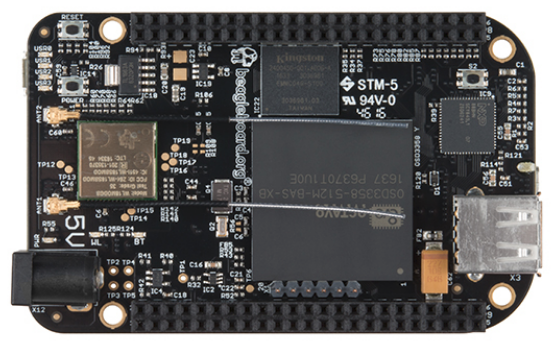
\includegraphics[scale=0.25]{img/mean/beaglebone-black-wireless.png}
        	\caption{Beaglebone black wireless}
        	\label{Beaglebone black wireless}
    	\end{figure}
\begin{center}
\textbf{\color{red}Hardware specifications : } 
A datasheet is available at {\color{blue}\url{https://www.alliedelec.com/m/d/5505861ee370de1c82065dcc7bc77b0c.PDF}}.
\end{center}

\subsubsection{Raspberry PI 3 B+}
The lastest version as this time of writing with enhanced processor and ethernet speed (\textbf{Figure \ref{Raspberry PI 3}}).
		\begin{figure}[H]
			\centering
        	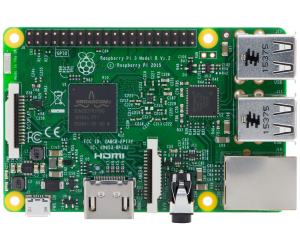
\includegraphics[scale=0.32]{img/mean/rpi3.png}
        	\caption{Raspberry PI 3}
        	\label{Raspberry PI 3}
    	\end{figure}
    	
\begin{center}	
\textbf{\color{red}Hardware specifications : } 
A datasheet is available at {\color{blue}\url{https://static.raspberrypi.org/files/product-briefs/Raspberry-Pi-Model-Bplus-Product-Brief.pdf}}.
\end{center}


\subsubsection{stm32f407 Board : } Used to build high performance applications oriented for audio processing (see \textbf{Figure \ref{stm32f407 Board}}).  
		\begin{figure}[H]
			\centering
        	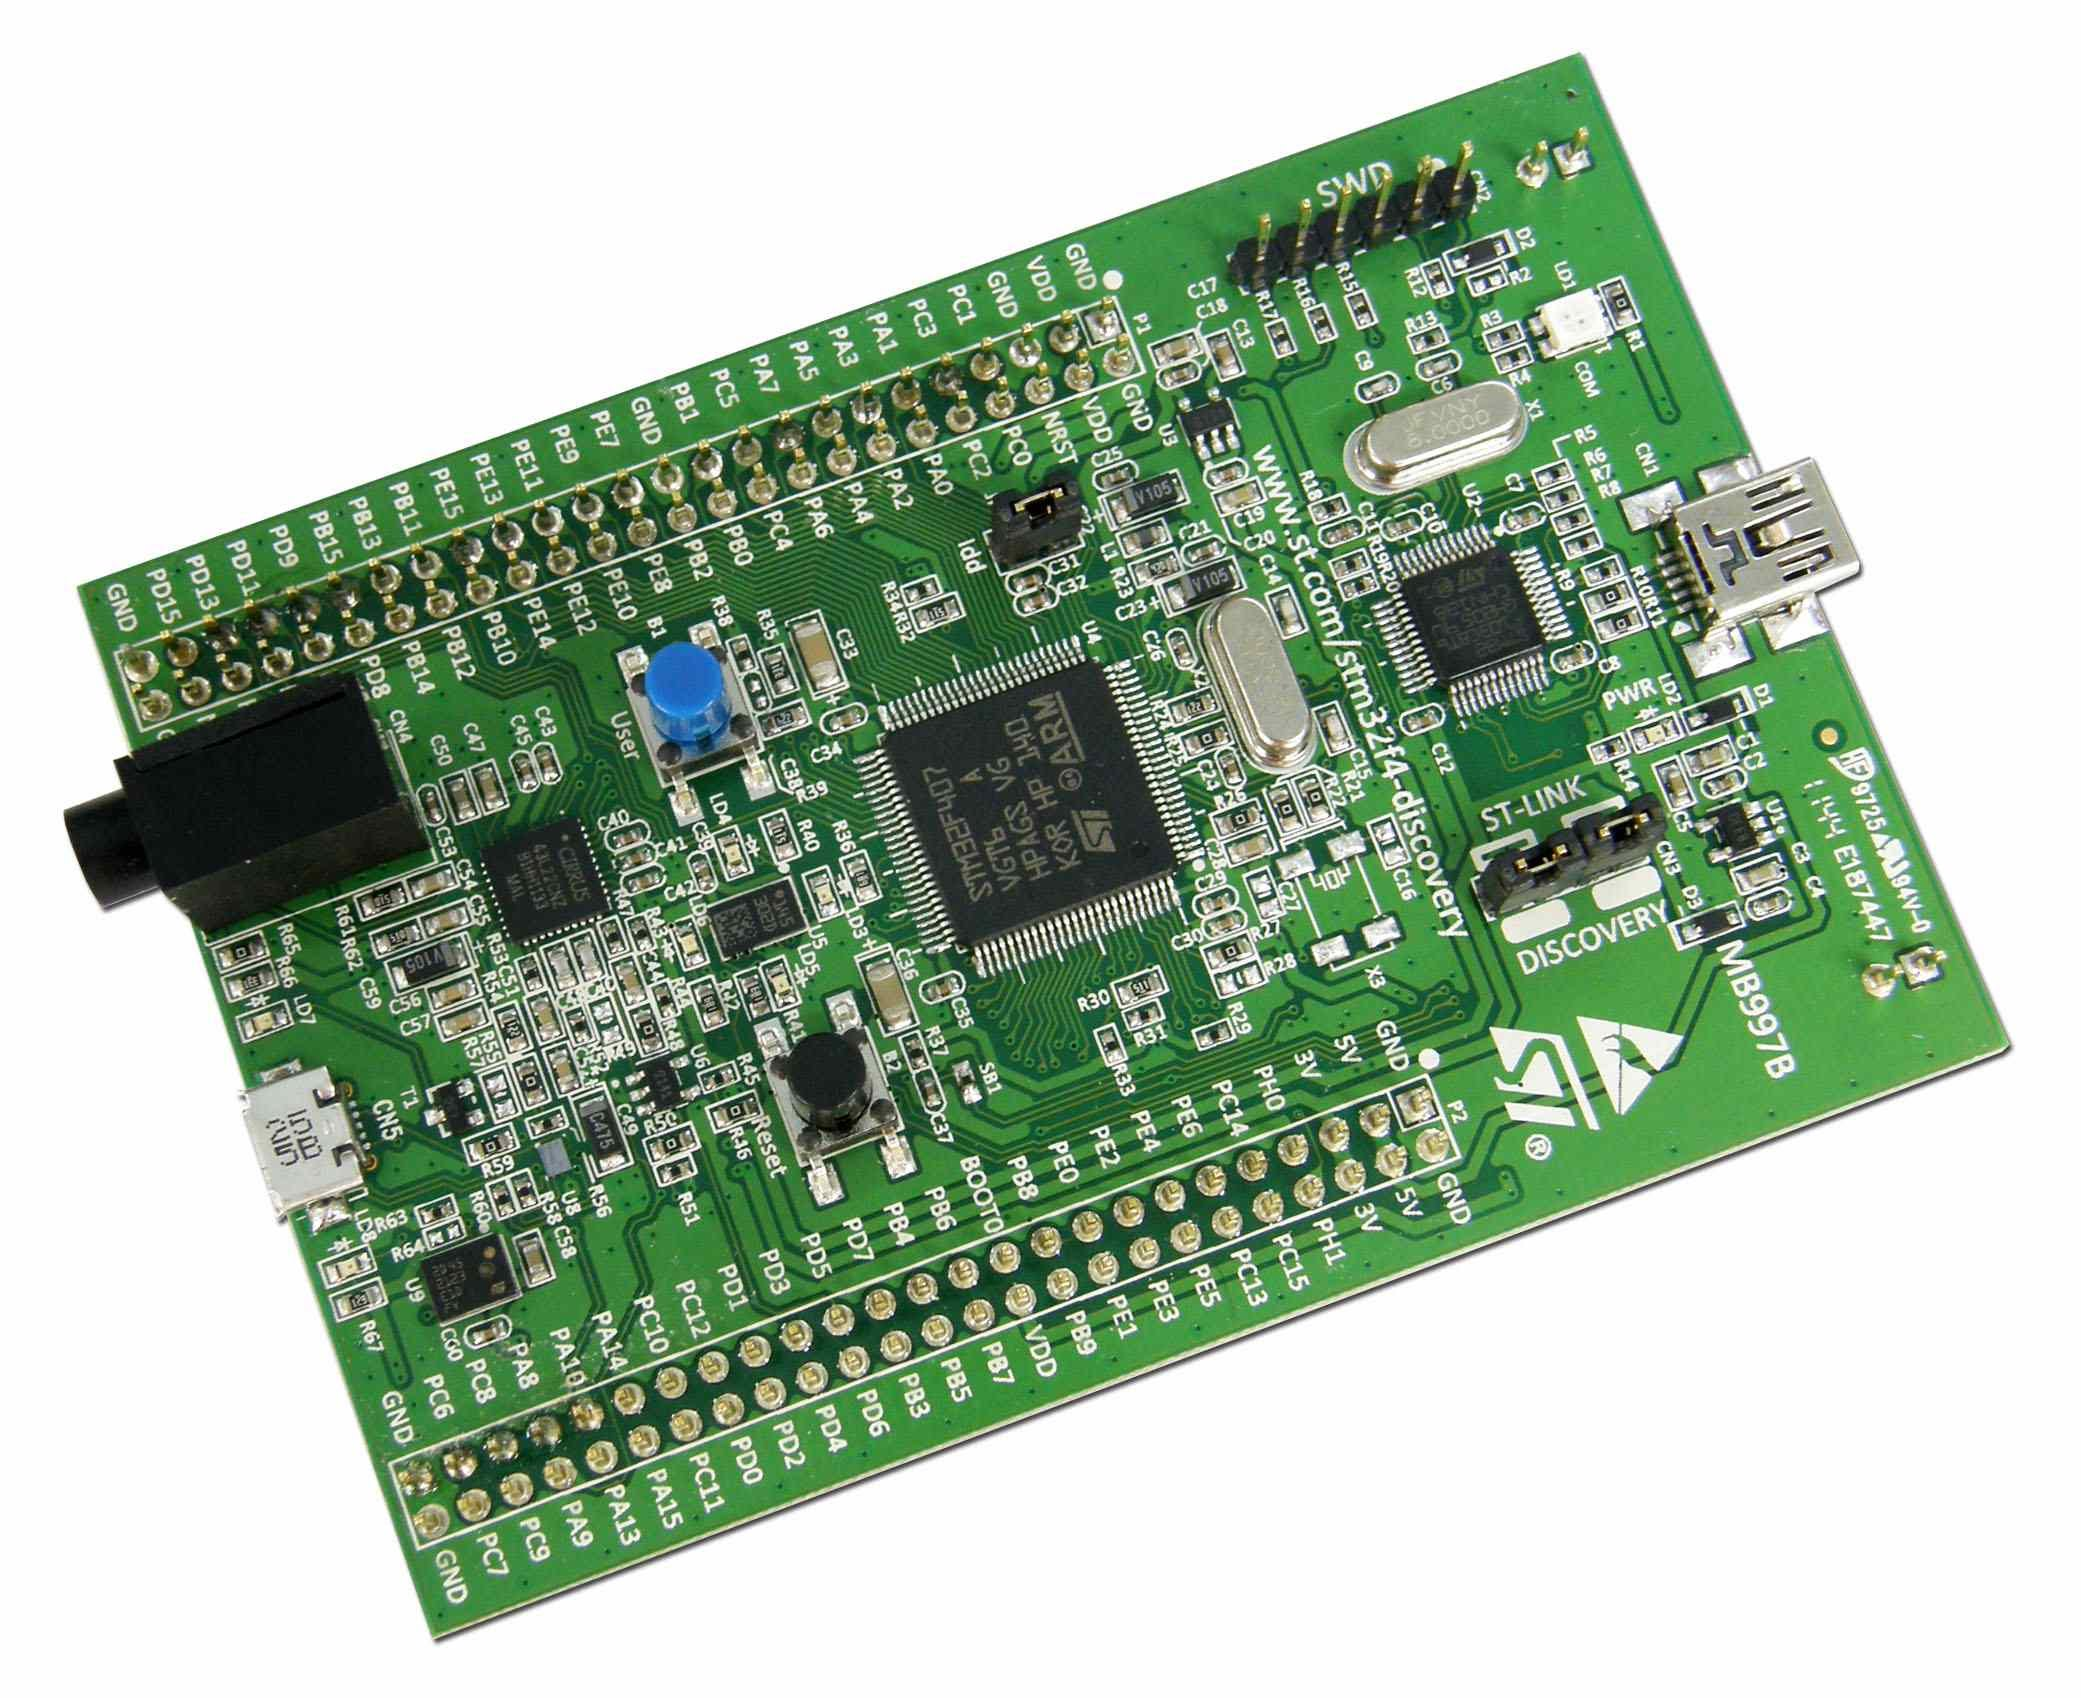
\includegraphics[scale=0.08]{img/mean/stm-32.jpg}
        	\caption{stm32f407 Board}
        	\label{stm32f407 Board}
    	\end{figure}
    	
\textbf{\color{red}Specifications are available at :} can be found at {\color{blue}\url{https://www.st.com/content/ccc/resource/technical/document/user_manual/70/fe/4a/3f/e7/e1/4f/7d/DM00039084.pdf/files/DM00039084.pdf/jcr:content/translations/en.DM00039084.pdf}}    	


\subsubsection{AT32UC3C-EK Board : }
An old developement kit for Atmel AVR microcontrolers (see \textbf{Figure \ref{AT32UC3C Board}}).  
		\begin{figure}[H]
			\centering
        	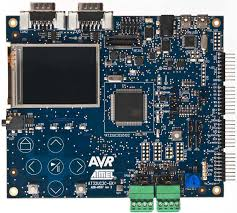
\includegraphics[scale=0.40]{img/mean/avr32.jpeg}
        	\caption{AT32UC3C Board}
        	\label{AT32UC3C Board}
    	\end{figure}
    	
    	\textbf{\color{red}Hardware spefications :}  available at {\color{blue}\url{http://www.farnell.com/datasheets/1511964.pdf}}

\subsubsection{ARM-USB-TINY-H JTAG Adapter : }  OpenOCD debugging interface adapter that uses the FTDI protocol (see \textbf{Figure \ref{ARM-USB-TINY-H}}).
		\begin{figure}[H]
			\centering
        	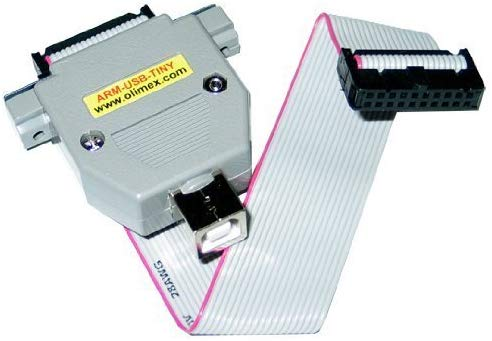
\includegraphics[scale=0.25]{img/mean/arm-usb-tiny-h.jpg}
        	\caption{ARM-USB-TINY-H}
        	\label{ARM-USB-TINY-H}
    	\end{figure}
Usage is described at : {\color{blue}\url{https://www.olimex.com/Products/ARM/JTAG/_resources/ARM-USB-TINY_and_TINY_H_manual.pdf}}\\

\textbf{\color{orange}Note : } OpenOCD supports multiple adapter protocols (ftdi, cmsis-dap, amt\_jtagaccel, remote\_bitbang, ..., etc). We can check the complet list at : {\color{blue}\url{http://openocd.org/doc/html/Debug-Adapter-Configuration.html#Debug-Adapter-Configuration}}. 
\subsection{Software}


\subsubsection{Pycharm IDE}
Pycharm is a python IDE, which makes developement fast. Examples of projects developed made in Python is an \textbf{OpenOCD wrapper} utility \og OESdebug \fg at : {\color{blue}\url{https://github.com/jugurthab/Linux_kernel_debug/tree/master/DebugSoftware/OpenOCD-wrapper}}.
\subsubsection{Eclipse C/C++ IDE}
Code examples were written maily in C, Eclipse C/C++ was helpful. Code are hosted on github at : {\color{blue}\url{https://github.com/jugurthab/Linux_kernel_debug/tree/master/debug-examples}}.

\subsubsection{OpenOCD}
Open source software allowing Hardware debugging, sources at maintained at : {\color{blue}\url{https://sourceforge.net/projects/openocd/files/openocd/}}.


\section{Internship solutions summary}
The following section discusses results of my intership. We are going to highlight the main points and illustrate with a couple of examples.

\begin{center}
\begin{mdframed}[
        linecolor=red,linewidth=2pt,% 
        frametitlerule=true,% 
        apptotikzsetting={\tikzset{mdfframetitlebackground/.append style={%
            shade,left color=white, right color=blue!20}}}, 
        frametitlerulecolor=blue,
        frametitlerulewidth=1pt, innertopmargin=\topskip,
        frametitle={About report},
        outerlinewidth=1.25pt
    ]
    % ----------
			This report gives only some samples of what was made, the entire project can be accessed at : {\color{blue}\url{https://github.com/jugurthab/Linux_kernel_debug}}.
			
			Full report (over 200 pages) is also available at : {\color{blue}\url{https://github.com/jugurthab/Linux_kernel_debug/blob/master/debugging-linux-kernel.pdf}}
\end{mdframed}
\end{center}




\subsection{Userspace}
Understading userspace bottlenecks is an everyday's job for every software developer, performance and even security engineer. Most appreciated debugging mechanisms were gathered as shown in \textbf{Figure \ref{Linux userspace debugging methodologies}}.
\begin{figure}[H]
		\centering
        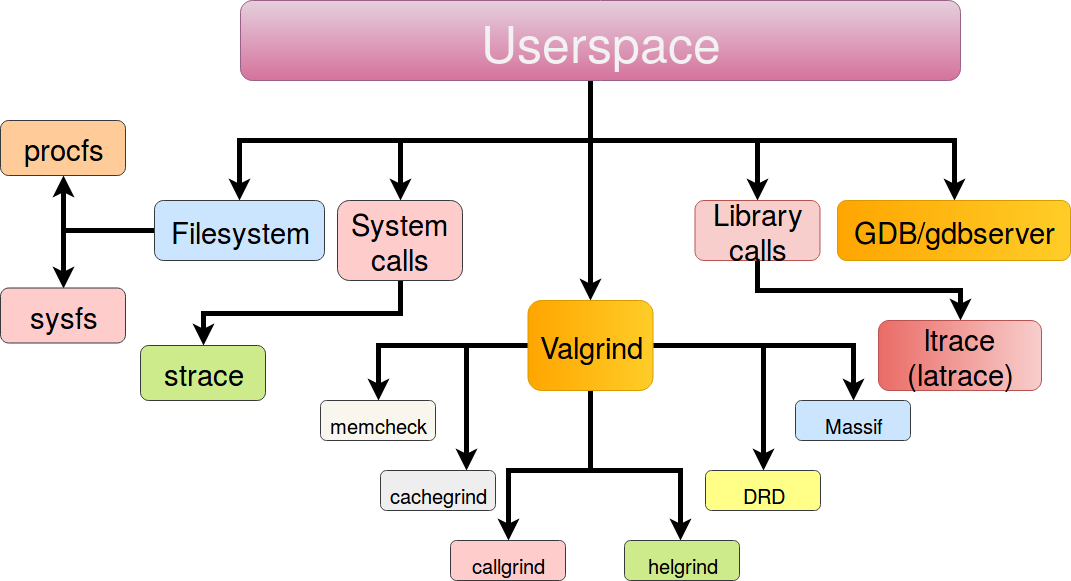
\includegraphics[scale=0.40]{img/solution/userspace.png}
        \caption{Linux userspace debugging methodologies}
        \label{Linux userspace debugging methodologies}
    \end{figure}
 
 
 
    
\textbf{\color{red}Important : } We are going to introduce each tool.
\subsubsection{Querying the filesystem}
\textbf{Linux} is enhanced in terms of security, robust and fault tolerant. It distinguishes between different level of privileges
and mainly : a \textbf{userspace} and \textbf{kernel-land}. This allows the system to correctly handle the resources and prevent unauthorized accesses.\\

However, there are important data-structures and information that we require even in userspace (\emph{memory allocated}, \emph{available resources}, \emph{state of process}, ..., etc). \textbf{Linux} provides us with two pseudo filesystems (\textit{because they do not exist on disk, they are created during system's boot}) that allow the kernel to share some it's knowledge to the userspace.    

\begin{itemize}
	\item \textbf{ProcFs : } exposes information related to processes (\emph{from which the name /proc stands for processes}) and system's configuration. Some interesting files for debugging :
		\begin{itemize}
			\item[$\bullet$] \textbf{/proc/pid/maps : } displays virtual address space layout of a given process (\textit{identified by pid}).
			\item[$\bullet$] \textbf{/proc/pid/status : } returns process specific informations (\emph{process status}, \emph{{\color{red}attached debugger}}, ..., etc).
			\item[$\bullet$] \textbf{/proc/pid/limits : }						
		\end{itemize}
Other files can be also helpful like : \textbf{/proc/meminfo} and \textbf{/proc/cpuinfo} which returns information associated to memory and processors respectively.	
	\item \textbf{SysFs : } a more recent filesystem (\emph{more organized than \textbf{procfs}}), We will be concerned with folder \textbf{/sys/module} as it is required to debug modules (\textit{as We will see later}). 
	
	
\end{itemize}

\subsubsection{System calls and library calls}
\label{System calls and library calls}
\textbf{Ptrace} is the most valuable mechanism to debug userspace applications. Most of utilities that are covered later (\emph{strace}, \emph{ltrace} and \emph{GDB}) rely on \textbf{ptrace} in the background (\emph{without it they will be useless}).\\

However, attackers uses it extensively too to escalate privileges.
Due to security issues, some distributions like \textbf{\color{red}Ubuntu disables ptrace} by default, We must enable it as follow :

\begin{lstlisting}[style=BashInputStyle]
$ sudo echo 0 > /proc/sys/kernel/yama/ptrace_scope
\end{lstlisting}

\begin{itemize}
	\item \textbf{System calls (Syscalls) : }
	strace is a debugging and diagnostic tool. The \og s \fg stands for \og system call \fg, which means that strace can monitor
Syscalls and reports them to end users.

An example is provided at : {\color{blue}\url{https://github.com/jugurthab/Linux_kernel_debug/tree/master/debug-examples/Chap1-userland-debug/strace}}

	\item \textbf{library calls : }
	Another successful tool is \og ltrace \fg which can record calls made from a binary executable file to shared libraries. \emph{It may save hours of debugging if used correctly}.
	
We have made an example at : {\color{blue}\url{https://github.com/jugurthab/Linux_kernel_debug/tree/master/debug-examples/Chap1-userland-debug/ltrace}}
\end{itemize}

ltrace has some limitations as it cannot trace calls amongst libraries. For this purpose, one need to use latrace (\textbf{Figure \ref{Catching executable to library and library to library calls - latrace}}).

\begin{figure}[H]
		\centering
        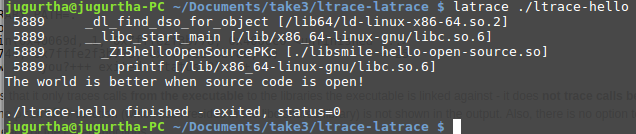
\includegraphics[scale=0.40]{img/solution/latrace-output.png}
        \caption{Catching executable to library and library to library calls - latrace}
        \label{Catching executable to library and library to library calls - latrace}
    \end{figure}



\textbf{Figure \ref{Comparing between strace, ltrace and latrace}} summarizes the differences between : \textbf{strace}, \textbf{ltrace} and \textbf{latrace}. 
\begin{figure}[H]
		\centering
        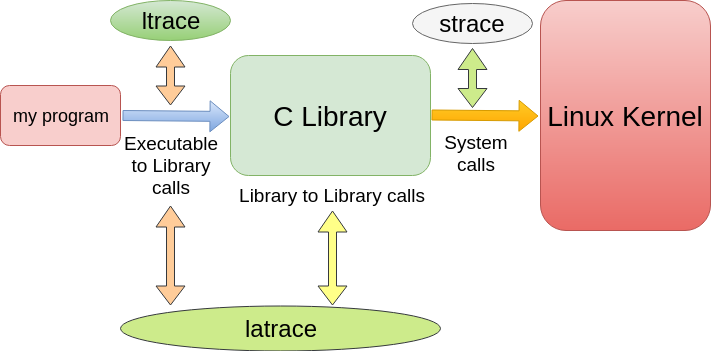
\includegraphics[scale=0.40]{img/solution/strace-ltrace-latrace.png}
        \caption{Comparing between strace, ltrace and latrace}
        \label{Comparing between strace, ltrace and latrace}
    \end{figure}


\subsubsection{Valgrind}
\textbf{Valgrind} is one of the most efficient memory debugging, intrumentation and profiling framework for userspace applications.
\begin{itemize}
	\item \textbf{memcheck : } default tool used by valgrind's engine. It can detect memory leaks, uninitialized variables, Mismatch allocation and deallocation functions (using malloc then free), Reading or writing past-off buffer, ..., etc (see {\color{blue}\url{https://github.com/jugurthab/Linux_kernel_debug/tree/master/debug-examples/Chap1-userland-debug/valgrind/memcheck}}).\\
	
The following record was taken from a report generated by memcheck which locates precisely the memory leak source (40 bytes lost at \textbf{memcheck-memory-leak.c:8}) :

		\begin{lstlisting}[style=BashInputStyle]
pi@raspberrypi:~/userspace/valgrind/memcheck$ valgrind --tool=memcheck \
> --leak-check=full ./memcheck-memory-leak 
==7369== Memcheck, a memory error detector
........................
==7369== HEAP SUMMARY:
==7369==     in use at exit: 40 bytes in 1 blocks
==7369==   total heap usage: 1 allocs, 0 frees, 40 bytes allocated
==7369== 
==7369== 40 bytes in 1 blocks are definitely lost in loss record 1 of 1
==7369==    at 0x4C2FB55: calloc (in /usr/lib/valgrind/vgpreload_memcheck-
amd64-linux.so)
==7369==    by 0x40053C: main (memcheck-memory-leak.c:8)
==7369== 
		\end{lstlisting}
	
	\item \textbf{helgrind : } a thread profiler with great support for POSIX pthreads (see {\color{blue} \url{https://github.com/jugurthab/Linux_kernel_debug/tree/master/debug-examples/Chap1-userland-debug/valgrind/helgrind}})	
	
	\item \textbf{cachegrind : }
	Simulates program's to cache hierarchy interaction in the system. Chachegrind will always simulate two cache levels :
		\begin{enumerate}
			\item {\textbf{L1 Cache :} Broken down into \emph{L1Data} and \emph{L1Instruction}.}
			\item {\textbf{Unified L2 Cache :} Data and instructions are mixed together.}
		\end{enumerate}			
An example is shown at : {\color{blue}\url{https://github.com/jugurthab/Linux_kernel_debug/tree/master/debug-examples/Chap1-userland-debug/valgrind/cachegrind}}
	
	\item \textbf{callgrind : } \textbf{Callgrind} is a CPU profiler. The reader is probably familiar with GPROF. Howerver, GPROF is deprecated(it can neither support multithreaded applications nor understand system calls).
We have provided an example at : {\color{blue}\url{https://github.com/jugurthab/Linux_kernel_debug/tree/master/debug-examples/Chap1-userland-debug/valgrind/callgrind}}


\end{itemize}

\subsubsection{GDB and GDBserver}


\begin{itemize}
	\item \textbf{GDB : } official build-in debugger from GNU collection. It can  start a program for debugging or attach to an already running process. Basically, gdb offers options shown in \textbf{Figure \ref{Basic features of GDB}}:
\begin{figure}[H]
		\centering
        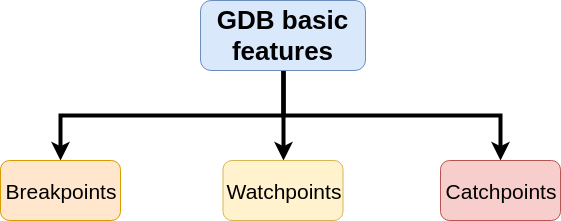
\includegraphics[scale=0.40]{img/solution/basic-usage-gdb.png}
        \caption{Basic features of GDB}
        \label{Basic features of GDB}
    \end{figure}	
	
\begin{itemize}
\item[$\bullet$] \textbf{Breakpoints : } are predefined points where GDB stops when it finds them in a program. They allow us to examine registers status,
memory dumps, environement variables, ..., etc (\textbf{Figure \ref{Setting GDB breapoints}}).
\begin{figure}[H]
		\centering
        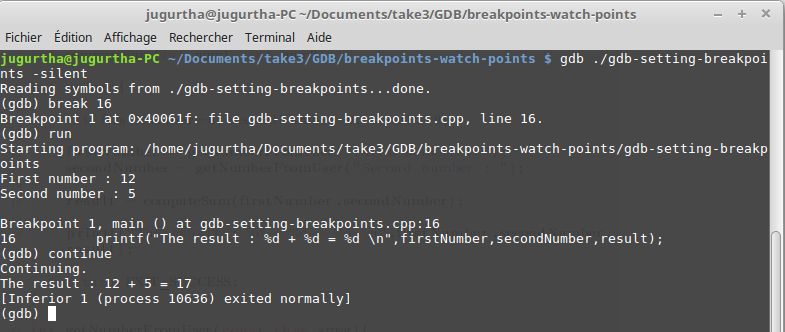
\includegraphics[scale=0.30]{img/solution/gdb-break-continue.png}
        \caption{Setting GDB breapoints}
        \label{Setting GDB breapoints}
    \end{figure}	



\item[$\bullet$] \textbf{Watchpoints : } can monitor a variable (read and write) and reports its status (\textbf{Figure \ref{Setting a read watchpoint in GDB}}).
\begin{figure}[H]
		\centering
        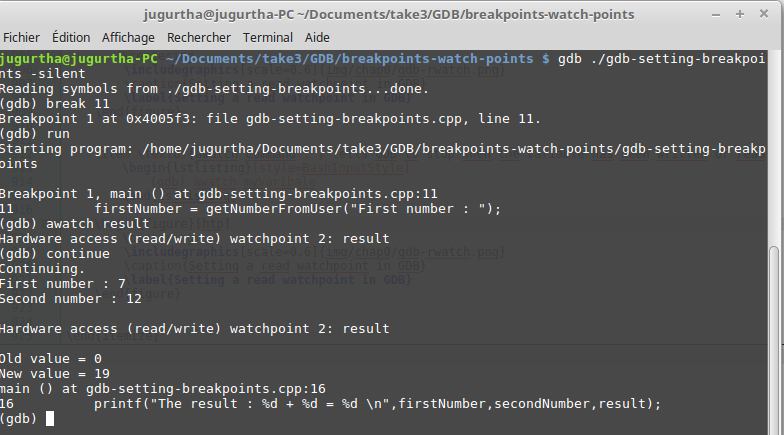
\includegraphics[scale=0.32]{img/solution/gdb-awatch.png}
        \caption{Setting a read watchpoint in GDB}
        \label{Setting a read watchpoint in GDB}
    \end{figure}
    
    
\item[$\bullet$] \textbf{Catchpoints : } report events like fork , signal reception (SIGUSER1,SIGALRM, ..., etc) and exceptions (\textbf{Figure \ref{Catching process forking using GDB}}).
\begin{figure}[H]
		\centering
        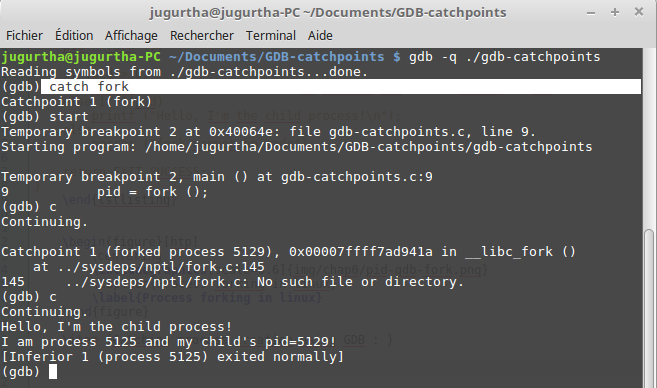
\includegraphics[scale=0.32]{img/solution/gdb-fork-got-catch.png}
        \caption{Catching process forking using GDB}
        \label{Catching process forking using GDB}
    \end{figure}
    


\end{itemize}	
	
	\item \textbf{GDBserver : }
	Local debugging is not always an option and may not be possible especially for embedded devices. Those systems
have fewer capabilities, a reason that leads us to remote debugging. \textbf{GDBserver} allows a program to be debugged remotely (\textbf{Figure \ref{Remote debugging using GDBserver}}).

\begin{figure}[H]
		\centering
        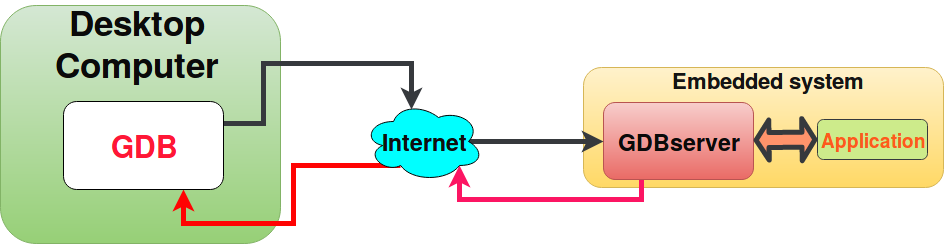
\includegraphics[scale=0.40]{img/solution/gdbAndGDBserver.png}
        \caption{Remote debugging using GDBserver}
        \label{Remote debugging using GDBserver}
    \end{figure}
\end{itemize}


Remote \textbf{GDBserver} accepts connections from both \emph{ethernet} and \emph{serial} communication : 
\begin{itemize}
	\item[$\ast$] \textbf{General settings of ethernet communication : } 
		\begin{enumerate}
			\item {GDBserver on the target}
						\begin{lstlisting}[style=BashInputStyle]
$ gdbserver :<portNumber> ./myProgram
						\end{lstlisting}
			\item {GDB Client - Linux machine side}
						\begin{lstlisting}[style=BashInputStyle]
$  gdb-cross-platform ./myProgram
$ (gdb) target remote ip_address_gdbserver_machine:<portNumber>
						\end{lstlisting}
						
		\end{enumerate}				
		
		
	\item[$\ast$] \textbf{General settings of serial communication : }	
		\begin{enumerate}
			\item {GDBserver on the target}
						\begin{lstlisting}[style=BashInputStyle]
$ gdbserver /dev/serial-channel ./myProgram
						\end{lstlisting}			
			\item {GDB Client - Linux machine side}
						\begin{lstlisting}[style=BashInputStyle]
$ gdb-cross-platform ./myProgram
$ (gdb) target remote /dev/serial-channel
						\end{lstlisting}	
		\end{enumerate}
\end{itemize}

	


Let's debug a \og \emph{Guess number} \fg program on a \textbf{Raspberry PI 3} running \textbf{GDBserver} \emph{(sources are available at : {\color{blue} \url{https://github.com/jugurthab/Linux_kernel_debug/tree/master/debug-examples/Chap1-userland-debug/gdb/remote-debug/raspberryPI3}})} : 
\begin{enumerate}
	\item \textbf{Raspberry PI 3 : } We will start Gdbserver on port 4000 (\emph{You can choose any other port}).
	\begin{lstlisting}[style=BashInputStyle]
$ gdbserver :4000 ./rpi-number-guess
    \end{lstlisting}

The result of the above command is shown in \textbf{Figure \ref{Starting gdbServer on Raspberry PI 3}}
\begin{figure}[H]
		\centering
        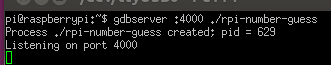
\includegraphics[scale=0.40]{img/solution/starting-ethernet-gdbserver-session-rp3.png}
        \caption{Starting gdbServer on Raspberry PI 3}
        \label{Starting gdbServer on Raspberry PI 3}
    \end{figure}



	\item \textbf{Linux desktop machine :} Launch a \textbf{gdb} session from a \textbf{Linux} machine and connect to target as shown in \textbf{Figure \ref{Rasbperry PI 3 - Remote debugging GDB/GDBserver over Ethernet}}
		\begin{lstlisting}[style=BashInputStyle]
$ ./arm-none-eabi-gdb -silent ./rpi-number-guess
$ (gdb) target remote ip_address_raspberryPI:4000	
    \end{lstlisting}
	
\begin{figure}[H]
		\centering
        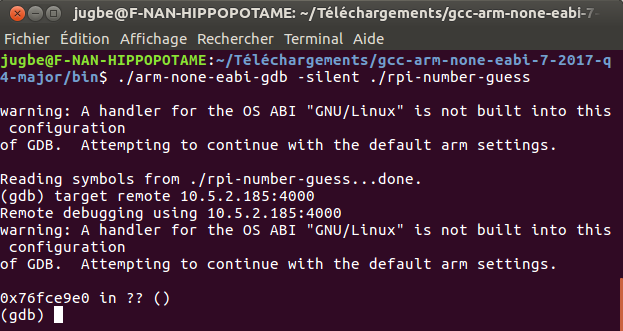
\includegraphics[scale=0.33]{img/solution/gdb-server-ethernet.png}
        \caption{Rasbperry PI 3 - Remote debugging GDB/GDBserver over Ethernet}
        \label{Rasbperry PI 3 - Remote debugging GDB/GDBserver over Ethernet}
    \end{figure}	
	
	At this point, a message sould be displayed at \textbf{Raspberry PI} side :
	
		\begin{lstlisting}[style=BashInputStyle]
Remote debugging from host ip_address_host_GDB	
    \end{lstlisting}
    
    
Now you can place breakpoints, move around (\emph{everything We know from GDB}) or even display generated number as shown in \textbf{Figure \ref{Displaying backtraces on Raspberry PI 3 using GDB/GDBserver over Ethernet}}    
\begin{figure}[H]
		\centering
        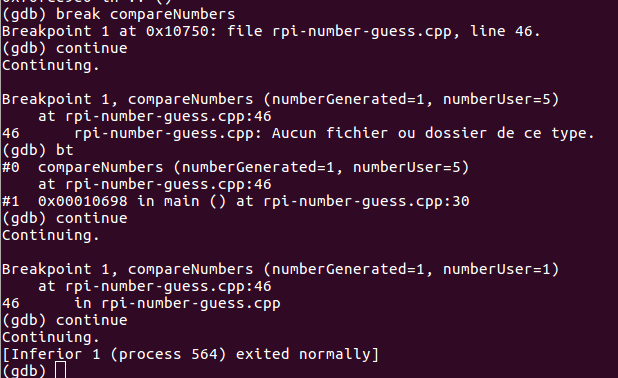
\includegraphics[scale=0.33]{img/solution/gdb-successfull-debug-over-ethernet.png}
        \caption{Displaying backtraces on Raspberry PI 3 using GDB/GDBserver over Ethernet}
        \label{Displaying backtraces on Raspberry PI 3 using GDB/GDBserver over Ethernet}
    \end{figure}    
    

\textbf{\color{orange}Note :} Latest versions of \textbf{Raspberry PI} seem to have troubles with Serial communication.	
\end{enumerate}

\subsubsection{File core dump}
When a userspace application was terminated abnormally (\emph{due to a segmentation fault for example}), the system saves the content of program's virtual memory space at the instant of termination for \textit{post analysis}, those files are known as \textbf{Core Dumps}.

\begin{enumerate}
	\item \textbf{Enabling file core crash : } core dumping is not available by default and it has to be enabled. Hopefully, we can change this easily as follow :
	
\begin{lstlisting}[style=BashInputStyle]	
$ ulimit -c unlimited
\end{lstlisting}	


	\item \textbf{Core crash generation : } Now, dump files are enabled; We can execute a faulty program:
\begin{lstlisting}[style=BashInputStyle]	
$ ./myProgram
Segmentation fault (core dumped)	
\end{lstlisting}
\textbf{Remark : } Notice the presence of \og core dump \fg which indicates a generated core dump.	
	\item \textbf{File crash core analysis : } GDB can be used to analyse the userspace crash dump files, all We have to do is to launch \textbf{GDB} as follow : 
\begin{lstlisting}[style=BashInputStyle]	
$ gdb ./myProgram <coreFile>	
\end{lstlisting}	


\textbf{\color{orange}Remember :} Your binary executable file must have been compilled with -g option, otherwise \textbf{GDB} is near to be useless.

	\item \textbf{Custumizing the name of the core file : }
	the default name of the core files is \og core \fg, but some problems may rise :
		\begin{itemize}
			\item {We may have multiple core files in such a way we cannot differentiate which core dump belongs to a particular
application}
			\item {If an application crashes multiple times, then the new core file will overwrite the old one.}
		\end{itemize}
		
		Linux provides two files to custumize the naming convetion of the core dumps :
		
		\begin{enumerate}
			\item \textbf{/proc/sys/kernel/core\_uses\_pid : } generates a core dump file named \og core.pid \fg, where pid is the identifier of the process being terminated. We can enable this feature by :
	\begin{lstlisting}[style=BashInputStyle]		
# echo 1 > /proc/sys/kernel/core_uses_pid			
\end{lstlisting}			
			\item \textbf{/proc/sys/kernel/core\_pattern : } allows to set a formated core dump files as shown below :
\begin{center}
	\begin{tabular}{|c|c|c|c|c|}
		\hline
		\rowcolor{LightCyan} 
			\textbf{Specifier} & \textbf{\%e} & \textbf{\%p} & \textbf{\%t} & \textbf{\%h}\\	   		
   		\hline
   		\textbf{Meaning} & Executable & process & timestamp & hostname\\
        	             & filename   & PID &  & \\
   		\hline
	\end{tabular}
\end{center}			
			
\textbf{\color{orange}Example :} let's save a core dump file with the naming format :	
	\begin{lstlisting}[style=BashInputStyle]
# echo core.%h.%e.%p.%t > /proc/sys/kernel/core_pattern
\end{lstlisting}	

Which results in a name : \og core.hostName.executableFileName.processID.timestamp \fg

Other specifiers exit like : \%u for real UID. The list is shown at : {\color{blue}\url{http://man7.org/linux/man-pages/man5/core.5.html}}.
		\end{enumerate}
\end{enumerate}

\subsection{Kernel land}
The kernel is more challenging to debug than userspace. Going through a code that changes a variable value (like userspace) is different from a kernel function that handles interrupts, manages memory, migrates tasks between processors, ..., etc.\\
\begin{center}
Weird behaviour should be expected when debugging kernel code
\end{center}  


\begin{figure}[H]
		\centering
        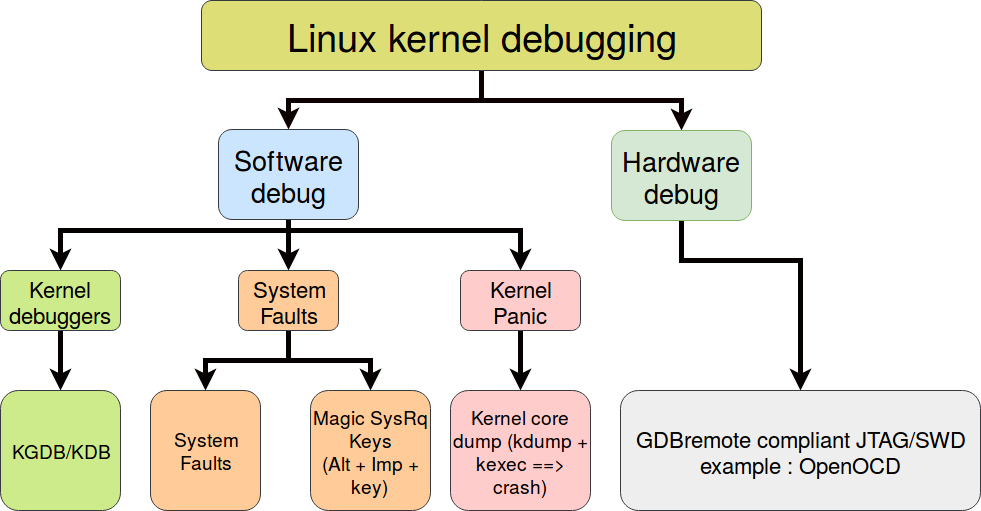
\includegraphics[scale=0.35]{img/solution/kernel-debugging-ways.png}
        \caption{Linux kernel debugging methodologies}
        \label{Linux kernel debugging methodologies}
    \end{figure}


\subsubsection{KGDB/KDB}
KGDB/KDB are the Linux kernel debuggers. KGDB is source level debugging and KDB is raw level.\\

The kernel must be built using special parameters in order to support KGDB/KDB as shown below :
\begin{itemize}
	\item \textbf{KGDB : } for KGDB support, the kernel must be compiled with : 
\begin{lstlisting}[style=BashInputStyle]
CONFIG_FRAME_POINTER=y
CONFIG_KGDB=y
CONFIG_KGDB_SERIAL_CONSOLE=y
\end{lstlisting}


	\item \textbf{KDB : } requires the following flags to be enabled :
\begin{lstlisting}[style=BashInputStyle]	
CONFIG_FRAME_POINTER=y
CONFIG_KGDB=y
CONFIG_KGDB_SERIAL_CONSOLE=y
CONFIG_KGDB_KDB=y
CONFIG_KDB_KEYBOARD=y
\end{lstlisting}	

\end{itemize}

\textbf{\color{orange}Note : } Kernel must be compiled with \textbf{\color{red}debugging symbols}, otherwise \textbf{KGDB}/\textbf{KDB} will be almost useless.


Important : We can check for KGDB/KDB support by reading /boot/config file. If this file is missing, one need to look for manufacturer documentation. \textbf{Figure \ref{Check for KGDB support on Raspberry PI 3}} shows how to check \textbf{KGDB}/\textbf{KDB} support on Raspberry PI 3.
\begin{figure}[H]
		\centering
        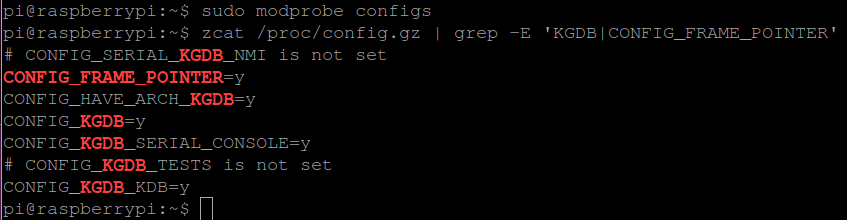
\includegraphics[scale=0.35]{img/solution/kgdb-support-raspberry-pi-3.png}
        \caption{Check for KGDB support on Raspberry PI 3}
        \label{Check for KGDB support on Raspberry PI 3}
\end{figure}

 

Both KGDB and KDB can be enabled by writing to the same file as illustrated :
\begin{lstlisting}[style=BashInputStyle]
pi@raspberrypi:~# echo ttyAMA0 > /sys/module/kgdboc/parameters/kgdboc
pi@raspberrypi:~# echo g > /proc/sysrq -trigger
\end{lstlisting}


Once \textbf{KGDB/KDB} is configured on the target, We can connect to the target in two different ways :

\begin{enumerate}
	\item \textbf{GDB : } connection will be established with \textbf{KGDB} on the target.
	
	\item \textbf{telnet : } connection will be received by \textbf{KDB} on the target (an example is shown in \textbf{Figure \ref{Debugging Beaglebone black wireless using KDB}}).
	
	\begin{figure}[H]
		\centering
        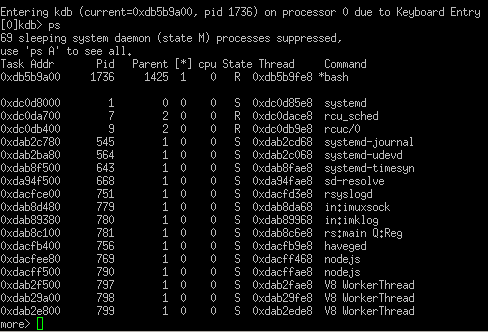
\includegraphics[scale=0.45]{img/solution/kdb-beagle-bone-black.png}
        \caption{Listing active processes on Beaglebone black wireless - KDB}
        \label{Debugging Beaglebone black wireless using KDB}
\end{figure}
	
	
\end{enumerate}

\subsubsection{System faults}
\textbf{System faults} does not mean \og panic \fg. Kernel Panic is a result of serious fault or a cascading effect of faults that can harm the system.\\
When a userspace program violates a memory access, a \emph{SIGSEGV} is generated and the faulty process is killed (remember to enable core dump files in order to analyse them). The same is true for the kernel, when a driver tries to dereference an invalid Null pointer or overflows the destination Buffer, it is going to be killed.\\


Buggy code in a driver or a module may lead to one of the states : \textbf{kernel oops} and \textbf{System Hang}.\\
\vspace{8px}

\begin{itemize}
	\item \textbf{Kernel oops : } Sometimes called \emph{Soft panics} (as opposed to hard kernel panic). Generally, they result from dereferencing a NULL pointer, overflowing kernel buffers and others faulty kernel code.\\
\vspace{5px}	


\begin{center}
\begin{mdframed}[
        linecolor=red,linewidth=2pt,% 
        frametitlerule=true,% 
        apptotikzsetting={\tikzset{mdfframetitlebackground/.append style={%
            shade,left color=white, right color=blue!20}}}, 
        frametitlerulecolor=blue,
        frametitlerulewidth=1pt, innertopmargin=\topskip,
        frametitle={Reading Kernel Oop},
        outerlinewidth=1.25pt
    ]
    % ----------
Kernel oops can be obtained by reading kernel's ring buffer with : \og \textbf{dmesg} \fg.
\end{mdframed}
\end{center}
	
\vspace{6px}	
We are going to take a look at 2 particular messages (We have provided a more detailed page at {\color{blue}\url{http://fdeszffffffffff}}) : 	

	\begin{enumerate}
		\item \textbf{Error location and type : } The kernel is really accurate in describing the problem (see \textbf{Figure \ref{Error type and location of faulty line - kernel oops}}).
		
\begin{figure}[H]
		\centering
        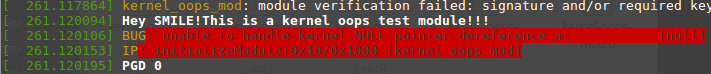
\includegraphics[scale=0.35]{img/solution/oops-error-kernel.png}
        \caption{Error type and location of faulty line - kernel oops}
        \label{Error type and location of faulty line - kernel oops}
    \end{figure}		
		
		
			\begin{itemize}
				\item \textbf{BUG : } shows the error name, in our case it \og dereferencing an NULL pointer\fg.				
				\item \textbf{IP : } Instrcution Pointer shows the location of the error (We will come back to it later).
			\end{itemize}					
		\item \textbf{Reason and number of oops : } oops may have cascading effect and lead to chain of oops (maybe even to kernel panic), the kernel identifies them and reports us the reason that gave rise to them as shown in \textbf{Figure \ref{Kernel Oops error code value - kernel oops}}.

		\begin{figure}[H]
			\centering
        	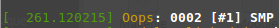
\includegraphics[scale=0.4]{img/solution/oops-error-kernel-smp.png}
        	\caption{Kernel Oops error code value - kernel oops}
        	\label{Kernel Oops error code value - kernel oops}
    \end{figure}
   
The error code \og 0002 \fg must be converted to binary. To understand the interpretation of the code take a look at \textbf{Figure \ref{Interpreting kernel oops error code}}.    
    	\begin{figure}[H]
			\centering
        	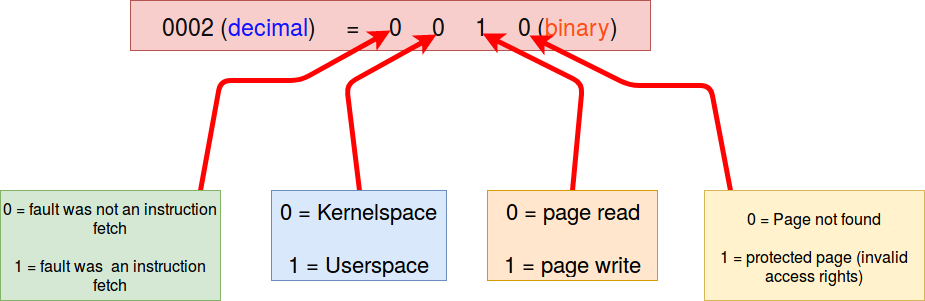
\includegraphics[scale=0.35]{img/solution/decodeKernelOops.png}
        	\caption{Interpreting kernel oops error code}
        	\label{Interpreting kernel oops error code}
    \end{figure}
    
  So finally, We can say that :  
    	\begin{center}
0 - 0 - 1 - 0 (binary) = a write request was made to a non existing page from the kernel and the instruction was not a \og fetch instruction \fg.    	
    	\end{center}
\textbf{\color{orange}Remark :} \textbf{\#1} shown in \textbf{Figure \ref{Kernel Oops error code value - kernel oops}} is the number of oops occurrence (\emph{As We have already said, the oops may happen multiple times and generate others}).
	\end{enumerate}
	
	\item \textbf{Kernel Hang and Magic Sysrq : }
	Everyone has experienced this situation at least one time. It is the state where a system is not responding anymore and completely frozen (not a KERNEL PANIC). This is called \textbf{\textit{Hang state}}.\\
	\vspace{5px}
Hopefully, We can use a forgotten feature in linux which is \textbf{SysRQ (Magic Keys)}.\\

\textbf{SysRQ} is combination of keyboard keys that executes a low level function. The kernel will always respond to \textbf{SysRQ}
whatever the state it is undergoing ; though, the only exception for this is \emph{kernel panic}.
\begin{center}
ALT + SysRq + <command key>
or
ALT + Print Screen + <command key>
\end{center}


\begin{center}
\begin{mdframed}[
        linecolor=red,linewidth=2pt,% 
        frametitlerule=true,% 
        apptotikzsetting={\tikzset{mdfframetitlebackground/.append style={%
            shade,left color=white, right color=blue!20}}}, 
        frametitlerulecolor=blue,
        frametitlerulewidth=1pt, innertopmargin=\topskip,
        frametitle={SysRq involves QWERTY Keyboard},
        outerlinewidth=1.25pt
    ]
    % ----------
		The kernel pretends a \textbf{QWERTY} keyboard when using \textbf{SysRq}.
\end{mdframed}
\end{center}


\vspace{10px}

SysRq are not enabled by default on some systems (especially the old ones), they must be activated :

	\begin{lstlisting}[style=BashInputStyle]
# echo 1 > /proc/sys/kernel/sysrq
	\end{lstlisting}
	
	\begin{itemize}
		\item[$\bullet$] \textbf{ALT + SysRq (Print Screen) + l :} shows the backtraces for all CPUs.
		
    \begin{figure}[H]
			\centering
        	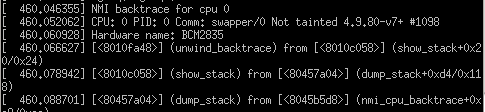
\includegraphics[scale=0.45]{img/solution/alt-sysrq-l.png}
        	\caption{Displaying backtraces for all CPUs using SysRq - Raspberry PI 3}
        	\label{Displaying backtraces for all CPUs using SysRq - Raspberry PI 3}
    \end{figure}		
		
		
		\item[$\bullet$] \textbf{ALT + SysRq (Print Screen) + m :} prints memory dump
		\item[$\bullet$] \textbf{ALT + SysRq (Print Screen) + p :} displays registers related information
		\item[$\bullet$] \textbf{ALT + SysRq (Print Screen) + c :} Forces a kernel panic, suitable if there is a \textbf{crashdump} utility installed on the system (\emph{more in the next section}).
	\end{itemize}
\end{itemize}



\textbf{\color{orange}Note :} \emph{\color{red}SysRq do not work on virtual machines (only some VM products support this feature), the combination of the key will be received by the HOST system.}

\subsubsection{Core dump and Kernel panic}
A kernel dump image can be obtained at any time in multiple ways. But, debugging symbols are mandatory.\\
If the kernel was not compiled using debugging symbols, one may try to add them as shown : {\color{blue}\url{https://www.ibm.com/support/knowledgecenter/en/linuxonibm/liacf/oprofkernelsymrhel.htm}}. Howerver, such packages are not always available. elfmaster came with a solution called kdress (but seems to work only on x86\_32 and x86\_64).


\begin{itemize}
	\item[$\bullet$] \textbf{Live kernel anaylysis /proc/kcore : }
		\begin{enumerate}
			\item \textbf{Generating vmlinux (optional) : } If the linux image was compiled without debugging symbols, We can try to construct them. \og kdress \fg was written by elfmaster is used for this purpose (kress is available at : {\color{blue}\url{https://github.com/elfmaster/kdress}}).
			
			
			\item \textbf{Accessing the /proc/kcore : }  We can play around the kcore using GDB, let's first create a GDB session as follow :
	\begin{lstlisting}[style=BashInputStyle]
# sudo gdb -q vmlinux /proc/kcore
	\end{lstlisting}			

			\item \textbf{Navigating through the /proc/kcore : } technically, We can obtain every information by walking through this file (see \textbf{Figure \ref{Navigating through /proc/kcore using gdb}}).
	
	\begin{figure}[H]
		\centering
        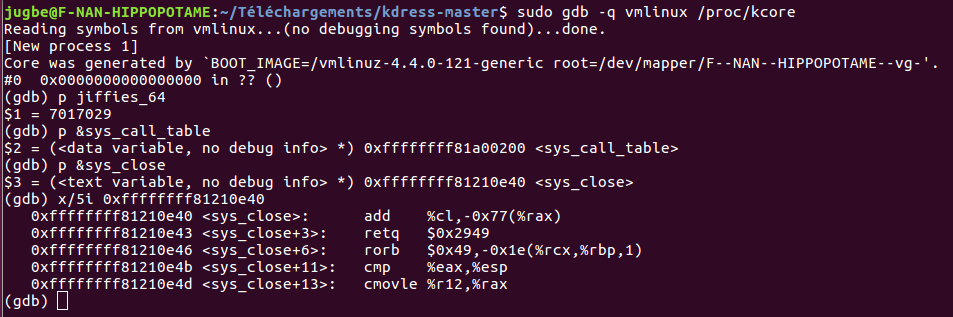
\includegraphics[scale=0.40]{img/solution/gdb-kcore-proc-navigation.png}
        \caption{Navigating through /proc/kcore using gdb}
        \label{Navigating through /proc/kcore using gdb}
    \end{figure}		
				
		\end{enumerate}
	\item[$\bullet$] \textbf{Post kernel crash analysis : } Kernel panic can be hard to troubleshoot (especially that bugs are almost impossible to reproduce in practice). We can get a kernel dump file in case of panic using Kdump and Kexec.
	
\begin{itemize}
	
	\item \textbf{kexec : } which allows to load quickly a new kernel from a running one (\textit{it does not perform any basic setup initialization like those made by BIOS}).
	\item \textbf{kdump : } uses kexec to start a new kernel when Panic is detected in the current one. Then dumps virtual memory (what can be dumped can be configured) of the crashed kernel from the newly launched one and saves result into a core dump file (can be stored in disk or sent through network which is ideal for embedded devices) as shown in \textbf{Figure \ref{Dumping Linux address space using kdump and kexec} - taken from Adrien Mahieux presentation- Linux crashdump analysis}. 
	\begin{figure}[H]
		\centering
        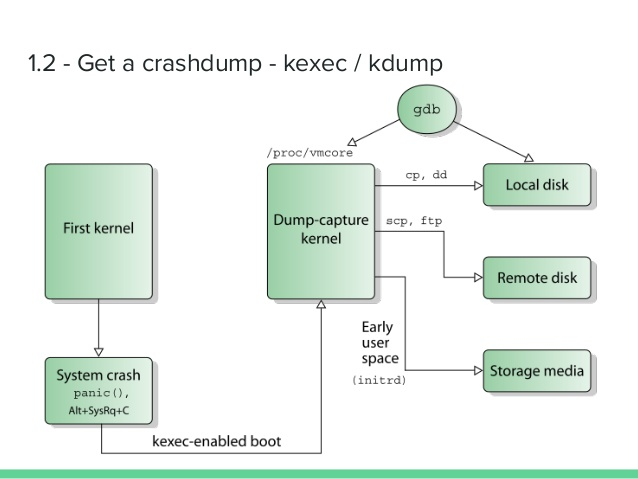
\includegraphics[scale=0.40]{img/solution/kdump-kexec.jpg}
        \caption{Dumping Linux address space using kdump and kexec}
        \label{Dumping Linux address space using kdump and kexec}
    \end{figure}

\end{itemize}




Once a dump file was generated, it can be analysed using GDB or a more specialized utlity like : crash.
	
\end{itemize}


\subsubsection{Linux hardware debugging with OpenOCD}
\label{Linux hardware debugging with OpenOCD}
\textbf{OpenOCD} is an open source project created by \og \textbf{Dominic Rath} \fg . It is supported by a large community which
maintains the source codes at {\color{blue}\url{https://sourceforge.net/projects/openocd/}}.\\
\textbf{OpenOCD} provides a high level abstraction to access a debugging hardware interface (\emph{JTAG}, \emph{SWD}, \emph{SPI}). Most
today's platforms have built-in JTAG connector which allows them to be {\color{green}inspected}, {\color{orange}tested} and even {\color{red}hacked}.

Let's summarize the working internals of OpenOCD : 

\begin{enumerate}
	\item \textbf{General overview of OpenOCD : } 
		\begin{figure}[H]
			\centering
        	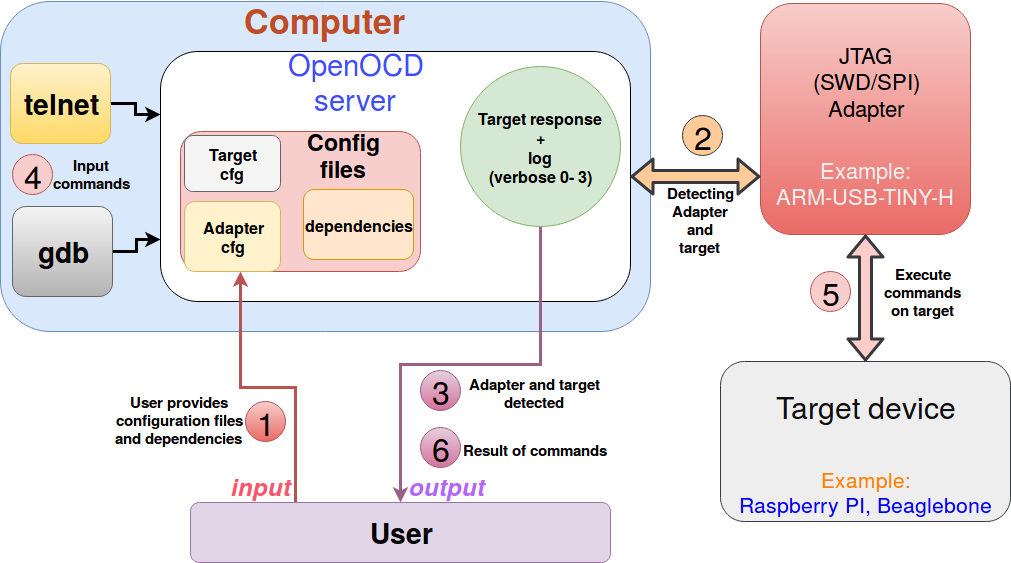
\includegraphics[scale=0.32]{img/solution/openOCDDiagram.png}
        	\caption{OpenOCD general settings}
        	\label{Navigating through /proc/kcore using gdb}
    	\end{figure}
	
		\begin{enumerate}
			\item {User starts OpenOCD with configuration files (at least adapter and target config files)}
			
			\item {If OpenOCD succeds to recognize the target, We can start debugging the target by using OpenOCD commands (OpenOCD receives commands from GDB or Telnet)}.
			
			\item {OpenOCD executes executes the commands on the target and returns back the result to the user}.
		\end{enumerate}		
	
	\item \textbf{General syntaxe Of OpenOCD : }	
	
	\begin{lstlisting}[style=BashInputStyle]	
$ sudo ./src/openocd -s tcl/ -f tcl/interface/adapter_config_file.cfg \ 
> -f tcl/target/target_config_file.cfg	
	\end{lstlisting}
		
		\begin{enumerate}
			\item \textbf{Hard wiring ARM-USB-TINY-H with raspeberry PI 3 : } connect Raspberry PI 3 with olimex JTAG adapter as shown in {Figure \ref{Connecting OpenOCD to Raspberry PI 3}}.
				\begin{figure}[H]
					\centering
        				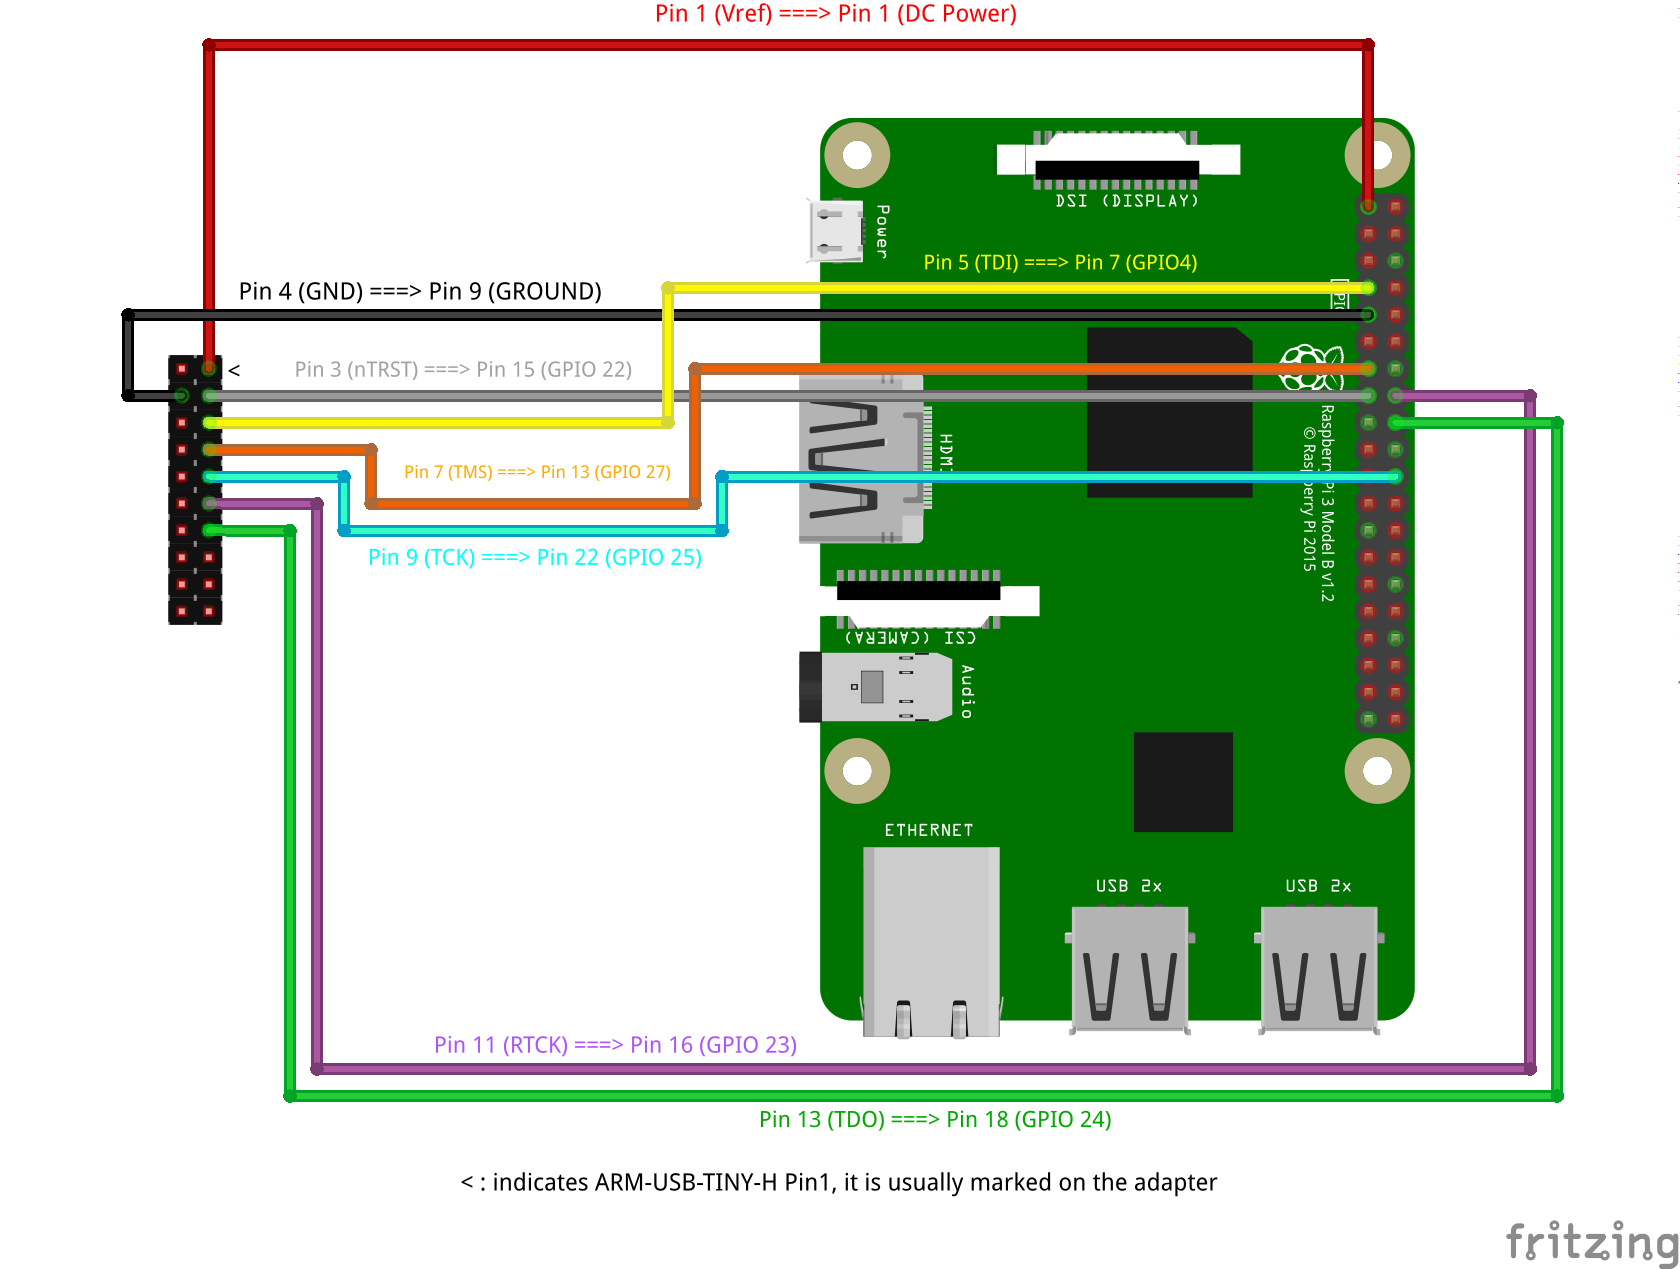
\includegraphics[scale=0.55]{img/solution/raspberry-PI-3-openocd-wiring.png}
        				\caption{Connecting OpenOCD to Raspberry PI 3}
        				\label{Connecting OpenOCD to Raspberry PI 3}
    			\end{figure}
    	
    		\item \textbf{Enabling JTAG on Raspberry PI 3 : }
    			\begin{itemize}
    				\item \textbf{Jtag enabler : } source code is available at : {\color{blue}\url{http://sysprogs.com/VisualKernel/legacy\_tutorials/raspberry/jtagsetup/JtagEnabler.cpp}}.
    				
    				\item \textbf{Edit Jtag enabler : } Jtag enablers seems to work only for Raspberry PI 1, the following lines should be changed as shown below :

		\begin{lstlisting}[style=CStyle]
#define BCM2708_PERI_BASE	0x3F000000
#define GPIO_BASE			(BCM2708_PERI_BASE + 0x200000)
		\end{lstlisting}
					\item \textbf{Execute Jtag enabler : } as shown \textbf{Figure \ref{Enable JTAG Debugging on Raspberry PI 3}}
					

		\begin{figure}[H]
			\centering
        	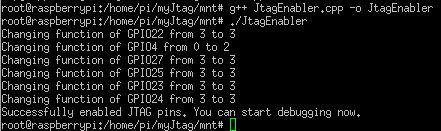
\includegraphics[scale=0.32]{img/solution/jtag-enabler-raspberry-pi-3.png}
        	\caption{Enable JTAG Debugging on Raspberry PI 3}
        	\label{Enable JTAG Debugging on Raspberry PI 3}
    	\end{figure}					
	
\textbf{\color{red}Important : } JTAG is enabled on Raspberry PI 3.	
					
    			\end{itemize}
    				
			\item \textbf{Debugging with OpenOCD : } We are ready to start \textbf{OpenOCD} as illustrated in \textbf{Figure \ref{Hardwiring ARM-USB-TINY-H to raspberry PI 3}}

		\begin{figure}[H]
			\centering
        	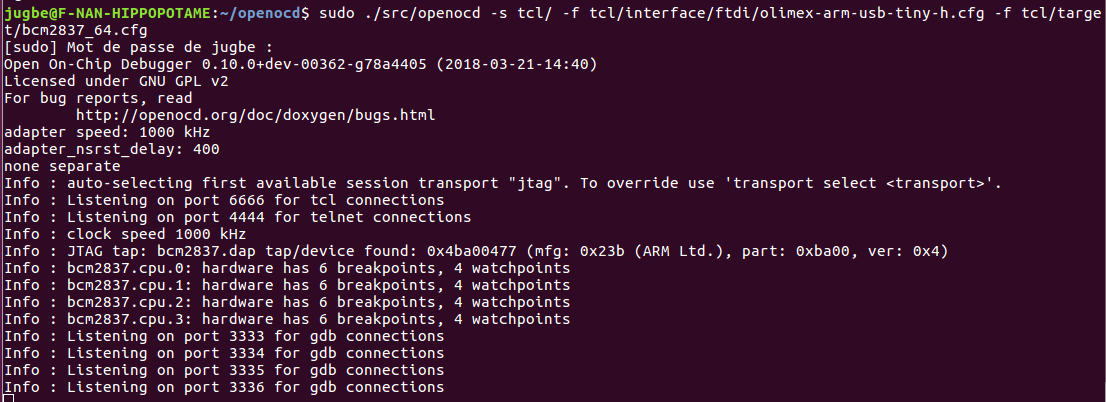
\includegraphics[scale=0.32]{img/solution/openocd-bcm2837-launched.png}
        	\caption{Hardwiring ARM-USB-TINY-H to raspberry PI 3}
        	\label{Hardwiring ARM-USB-TINY-H to raspberry PI 3}
    	\end{figure}	

	
	\textbf{\color{orange}Note :} the line \og \emph{Info : JTAG tap : bcm2837.dap tap/device found : 0x4ba00477 (mfg : 0x23b (ARM Ltd.), part :
0xba00, ver : 0x4)} \fg means that OpenOCD was able to detect the Raspberry PI 3. We also see the breakpoints which indicates highly that the connection was a success.
		\end{enumerate}
		
	
	
	\item \textbf{OpenOCD made easy with OESdebug : } OpenOCD is quiet difficult and complex to setup. We have provided a tool called \og OpenOCD-wrapper \fg (OpenEasy Debug is written in python3) as a high level wrapper around \textbf{OpenOCD}. \emph{It allows even to generate \textbf{OpenOCD} scripts on the fly}.\\
	\label{OpenOCD made easy with OESdebug}

\begin{center}
\begin{mdframed}[
        linecolor=red,linewidth=2pt,% 
        frametitlerule=true,% 
        apptotikzsetting={\tikzset{mdfframetitlebackground/.append style={%
            shade,left color=white, right color=blue!20}}}, 
        frametitlerulecolor=blue,
        frametitlerulewidth=1pt, innertopmargin=\topskip,
        frametitle={OESdebug sources},
        outerlinewidth=1.25pt
    ]
    % ----------
		Sources are available at : {\color{blue}\url{https://github.com/jugurthab/Linux_kernel_debug/tree/master/DebugSoftware/OpenOCD-wrapper}}.
\end{mdframed}
\end{center}

	
	
	\begin{enumerate}
		\item \textbf{Start OESdebug : } We only need python3 interpreter and python-tk (graphic's library to be installed) :
		\begin{lstlisting}[style=BashInputStyle]
# python3 main.py
	\end{lstlisting}	
			
	
		\item \textbf{OpenOCD support :} \textbf{OESdebug} is a wrapper program which intends to use OpenOCD easily. OESdebug checks for OpenOCD presence at start-up (\textit{one can pinpoint OpenOCD's location if compiled from sources}). \textbf{Figure \ref{Checking OpenOCD support - OESdebug}} shows OESdebug when OpenOCD is detected.		
		\begin{figure}[H]
			\centering
        	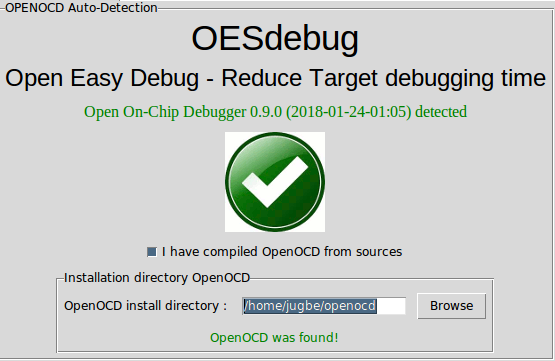
\includegraphics[scale=0.32]{img/solution/OESdebug-detect-OpenOCD.png}
        	\caption{Checking OpenOCD support - OESdebug}
        	\label{Checking OpenOCD support - OESdebug}
    	\end{figure}
		
			
		\item \textbf{Adapter Support : } an adapter is the intermidiate component that allows OpenOCD (running as a deamon in the host) to access the target's JTAG TAP controller. We must choose a supported adapter that ships with OpenOCD (as shown in \textbf{Figure \ref{Checking Adapter support - OESdebug}}) or create one (by checking \og create a custom adapter \fg).
		\begin{figure}[H]
			\centering
        	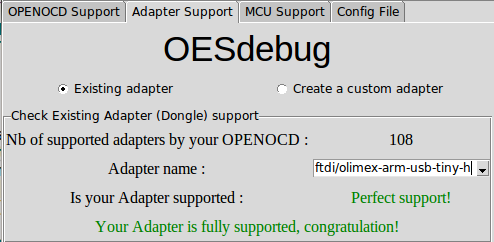
\includegraphics[scale=0.32]{img/solution/OESdebug-adapterSupport.png}
        	\caption{Checking Adapter support - OESdebug}
        	\label{Checking Adapter support - OESdebug}
    	\end{figure}
    			
		\item \textbf{MCU support : } OpenOCD cannot support every target that exists (\textit{We can add our own configuration file but it's a bit more enhanced} as shown in \textbf{Figure \ref{Creating a new target config file - OESdebug}}).
		\begin{figure}[H]
			\centering
        	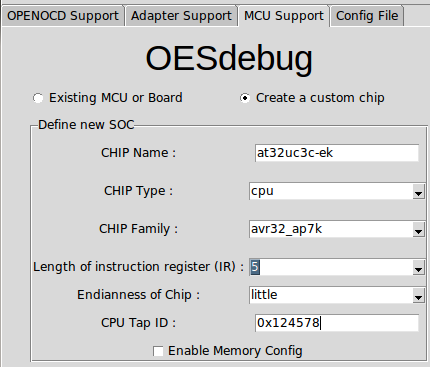
\includegraphics[scale=0.32]{img/solution/OESdebug-new-board.png}
        	\caption{Creating a new target config file - OESdebug}
        	\label{Creating a new target config file - OESdebug}
    	\end{figure}
    			
		\item \textbf{Generating configuration file : } Now, We can click on "Generate" to get a working OpenOCD script (\textbf{Figure \ref{Generating OpenOCD config file - OESdebug}}).
		\begin{figure}[H]
			\centering
        	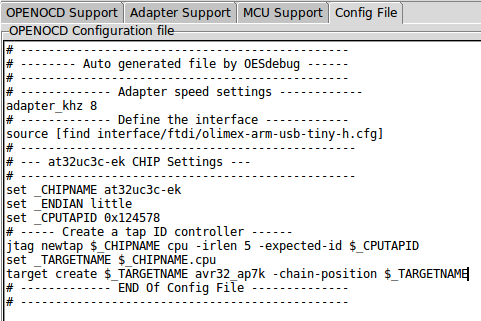
\includegraphics[scale=0.32]{img/solution/OESdebug-generatedScript.png}
        	\caption{Generating OpenOCD config file - OESdebug}
        	\label{Generating OpenOCD config file - OESdebug}
    	\end{figure}		
		
		
		\item \textbf{Launching OpenOCD : } Once script file is generated, We can start OpenOCD using start OpenOCD button. If the configuration was successful, OpenOCD will recognize the target as shown in \textbf{Figure \ref{Launching OpenOCD from OESdebug on AT32UC3C-EK target}}.		
		\begin{figure}[H]
			\centering
        	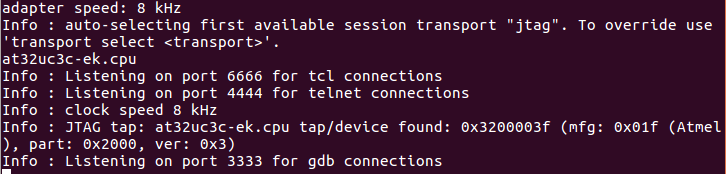
\includegraphics[scale=0.32]{img/solution/at32uc3c0512c-found-openocd.png}
        	\caption{Launching OpenOCD from OESdebug to debug AT32UC3C-EK target}
        	\label{Launching OpenOCD from OESdebug on AT32UC3C-EK target}
    	\end{figure}	
	
		The AT32UC3C-EK has been successfully detected by OpenOCD (\textit{because OpenOCD returned \textit{tap/device found}}).
		
\textbf{\color{orange}Note :} \textbf{OESdebug} defaults the adapter speed to 8 khz (\textit{always use this speed if not sure about adapter's communication speed}). 	 
\begin{center}
\begin{mdframed}[
        linecolor=red,linewidth=2pt,% 
        frametitlerule=true,% 
        apptotikzsetting={\tikzset{mdfframetitlebackground/.append style={%
            shade,left color=white, right color=blue!20}}}, 
        frametitlerulecolor=blue,
        frametitlerulewidth=1pt, innertopmargin=\topskip,
        frametitle={OESdebug Extra features},
        outerlinewidth=1.25pt
    ]
    % ----------
	\textbf{OESdebug} supports \textbf{Auto probing} (to get TAP ID and Intruction register length) and also \textbf{saving generated scripts}  to share them easily (\textit{see it's Help section}).
\end{mdframed}
\end{center}

	\end{enumerate}
	
	
		
\end{enumerate}
	



\subsection{Linux tracers}
Tracing is the opposite of security, if security wants to hide what's happening in the kernel than tracing does the complete opposite.

\subsubsection{Ftrace}
Ftrace is the official linux tracing tool created by \og \textbf{Steven Rostedt} \fg that has been merged to linux mainline since version \emph{2.6.31}.

\begin{itemize}
	\item[$\bullet$] \textbf{Trace-cmd : }
Ftrace is quite tedious, boring and requires a long setup before we can get a trace. The creator of Ftrace \og \textbf{Steven Rostedt} \fg released a Front-end tool for Ftrace called Trace-cmd.	

The general syntax used to record events using trace-cmd is :
	\begin{lstlisting}[style=BashInputStyle]
# trace-cmd record -p <tracer> -e <event1> -e <event2> -e <eventN> <program>
	\end{lstlisting}
	
And for reading events :
	\begin{lstlisting}[style=BashInputStyle]
# trace-cmd report
	\end{lstlisting}	

As a working example, We will are going to trace a module :
\begin{enumerate}
	\item \textbf{Loading module : } neverthless to say that before tracing the module, it must be running (\textbf{Figure \ref{Insertion of module to kernel before tracing}})
		\begin{figure}[H]
			\centering
        	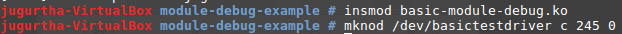
\includegraphics[scale=0.32]{img/solution/insert-your-module-to-kernel.png}
        	\caption{Insertion of module to kernel before tracing}
        	\label{Insertion of module to kernel before tracing}
    	\end{figure}
    		
	\item \textbf{Tracing module function : } We can launch trace-cmd, and set a filter on the functions to trace (in our case all function names that begin with \og basic \fg)
	
		\begin{figure}[H]
			\centering
        	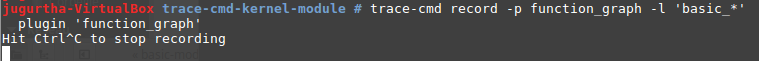
\includegraphics[scale=0.32]{img/solution/trace-cmd-tracing-module.png}
        	\caption{Tracing functions in a module using trace-cmd}
        	\label{Tracing functions in a module using trace-cmd}
    	\end{figure}	
	
	\item \textbf{Interact with the module : } after starting Ftrace, We must call one of the functions of our module. let's make a simple read on it (\textbf{Figure \ref{Interacting with the kernel device module}})
		\begin{figure}[H]
			\centering
        	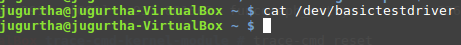
\includegraphics[scale=0.32]{img/solution/interacting-driver-trace-cmd.png}
        	\caption{Interacting with the kernel device module}
        	\label{Interacting with the kernel device module}
    	\end{figure}		
	
	
	\item \textbf{Reading report : } (\textbf{Figure \ref{Reading module trace report with Trace-cmd}})
			\begin{figure}[H]
			\centering
        	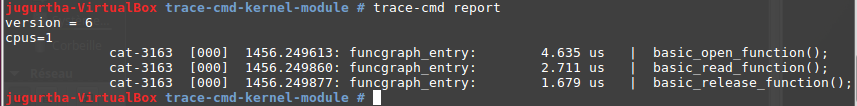
\includegraphics[scale=0.32]{img/solution/trace-cmd-report-module.png}
        	\caption{Reading module trace report with Trace-cmd}
        	\label{Reading module trace report with Trace-cmd}
    	\end{figure}		
	
	
	
\end{enumerate}

	
	
	\item[$\bullet$] \textbf{Kernelshark : }	
We cannot close the discussion about Ftrace without pointing out an important tool called \og Kernelshark \fg.
Reading Ftrace report can be quiet difficult ; the third tool released by \og \textbf{Steven Rostedt} \fg is KernelShark which is GUI based (an example is shown in \textbf{Figure \ref{Kernelshark shows process scheduling after parsing traces of a raspberry PI 3}}).

		\begin{figure}[H]
			\centering
        	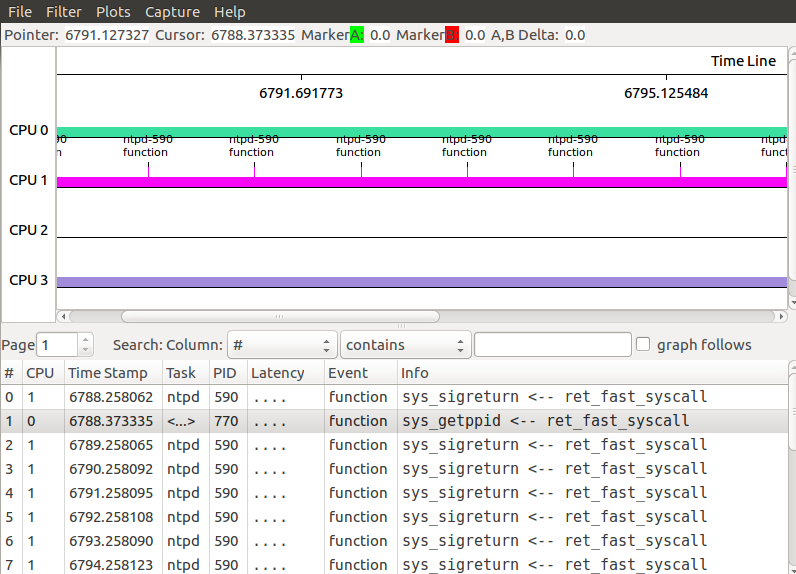
\includegraphics[scale=0.32]{img/solution/kernelshark-task-schedule.png}
        	\caption{Kernelshark shows process scheduling after parsing traces of a raspberry PI 3}
        	\label{Kernelshark shows process scheduling after parsing traces of a raspberry PI 3}
    	\end{figure}




\end{itemize}


\subsubsection{LTTng}


\begin{enumerate}
	\item \textbf{Create a session :} Every LTTng record must be made within a session (the session name can be anything We want) :
		\begin{lstlisting}[style=BashInputStyle]
# lttng create <mySessionName>
	\end{lstlisting}	

		\begin{figure}[H]
			\centering
        	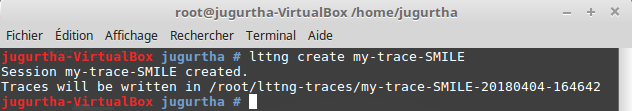
\includegraphics[scale=0.32]{img/solution/create-session-lttng.png}
        	\caption{Creating a session in LTTng}
        	\label{Creating a session in LTTng}
    	\end{figure}	
	
	
	\item \textbf{Select a tracepoint (instrumentation point) : } We may select one or multiple (or even all) tracepoints.\\
We will choose for example to trace \og sched\_switch \fg :

		\begin{figure}[H]
			\centering
        	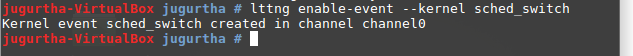
\includegraphics[scale=0.32]{img/solution/lttng-select-event.png}
        	\caption{Select kernel tracepoints in LTTng}
        	\label{Select kernel tracepoints in LTTng}
    	\end{figure}



	\item \textbf{Start the tracing session :} We can start tracing at this point, LTTng will record all \og sched\_switch \fg events
		\begin{figure}[H]
			\centering
        	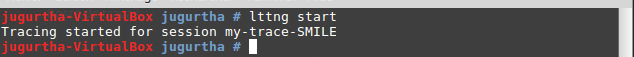
\includegraphics[scale=0.32]{img/solution/lttng-start-tracing.png}
        	\caption{Start tracing using LTTng}
        	\label{Start tracing using LTTng}
    	\end{figure}


	\item \textbf{Stop tracing session :} stop subcommand will halt recording and saves the tracing report.
		\begin{figure}[H]
			\centering
        	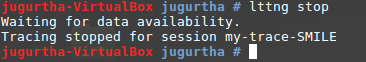
\includegraphics[scale=0.32]{img/solution/lttng-stop-session.png}
        	\caption{Stop tracing using LTTng}
        	\label{Stop tracing using LTTng}
    	\end{figure}
	
	\item \textbf{Destroy LTTng session :} We need to stop and destroy the current session.
			\begin{lstlisting}[style=BashInputStyle]
# lttng destroy
	\end{lstlisting}
	
		\item \textbf{Visualize the trace report : } 
		
			\begin{itemize}
				\item[$\bullet$] \textbf{babeltrace : } We can view LTTng report in the console, however, when We record a lot of events for a
long time, viewing the result in text-based mode is far to be easy
		\begin{figure}[H]
			\centering
        	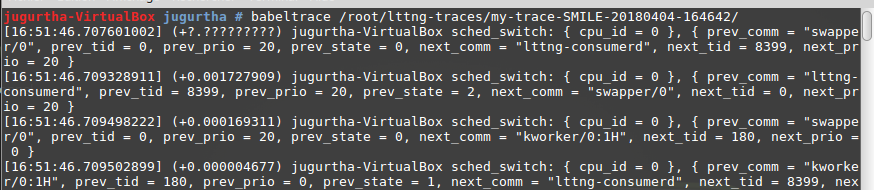
\includegraphics[scale=0.32]{img/solution/babel-trace.png}
        	\caption{Reading LTTng trace report using babeltrace}
        	\label{Reading LTTng trace report using babeltrace}
    	\end{figure}				
				
				
				\item[$\bullet$] \textbf{trace compass : } This is a visual GUI to display the LTTng traces in a more convinient way. \emph{\color{orange}Trace compass is an Eclipse C/C++ pluggin}.
			\end{itemize}
\end{enumerate}




We can say even more on LTTng : 
\begin{itemize}
	\item \textbf{LTTng USDT : } LTTng enables to attach User Statically Defined Tracepoints to userspace applications (\emph{something not possible using Ftrace or perf}). It can trace \textbf{C/C++} code (as shown at : \textbf{\color{blue}\url{https://github.com/jugurthab/Linux_kernel_debug/tree/master/debug-examples/Chap3-tracers/Lttng-examples/Tracing-Userspace-C-App}}), \textbf{Python} scripts ({\color{blue} \url{https://github.com/jugurthab/Linux_kernel_debug/tree/master/debug-examples/Chap3-tracers/Lttng-examples/Tracing-Userspace-Python-App}}) and even \textbf{Java}. 
	
	\item {LTTng Logger file : } when \textbf{LTTng} deamon is running (lttngd), it creates a special file in \textbf{ProFs} : \textbf{\color{red}\url{/proc/lttng-logger}}.
		Applications can log their messages to this file (usefull for debugging), however it is not reliable as \textbf{LTTng USDT}.
	
	\item \textbf{LTTng toolkit analyses : }
LTTng provides a powerfull toolkit called \og LTTng analyses \fg to extract most relevant data from recorded traces ({\color{blue} \url{https://github.com/lttng/lttng-analyses}}). We are going to show two examples :

		\begin{itemize}
			\item \textbf{lttng-analyses-record : } which record an automatic LTTng session (instead of manual recording as We did) as shown in \textbf{Figure \ref{Automatic session recording - LTTng toolkit analyses}}
					\begin{figure}[H]
						\centering
        				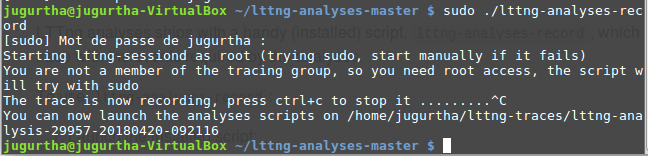
\includegraphics[scale=0.35]{img/solution/lttng-analyses-automatic-record.png}
        				\caption{Automatic session recording - LTTng toolkit analyses}
        				\label{Automatic session recording - LTTng toolkit analyses}
    				\end{figure}
			
			
			\item \textbf{lttng-schedlog : } shows task scheduling in chronogical order (\textbf{Figure \ref{Getting sched-switch logs from traces - LTTng toolkit analyses}}).
					\begin{figure}[H]
						\centering
        				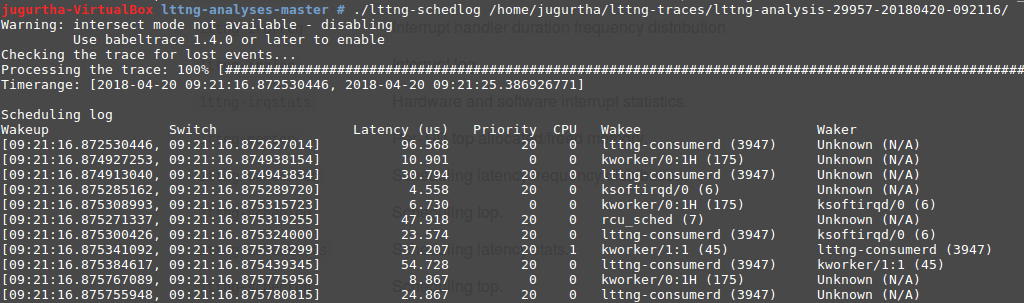
\includegraphics[scale=0.35]{img/solution/lttng-schedlog.png}
        				\caption{Getting sched\_switch logs from traces - LTTng toolkit analyses}
        				\label{Getting sched-switch logs from traces - LTTng toolkit analyses}
    				\end{figure}		
			
			
		\end{itemize}			
	
	
\end{itemize}


\subsubsection{Perf}
\textbf{Perf} is a linux official profiler, tracer and benchmarker tool that has been merged to the linux mainline since version 2.6.31.

The most perf's used commands are :
\begin{itemize}
	\item \textbf{list :} lists the events supported by perf (HW/SW events, tracepoints).
	\item \textbf{stat :} counts the number of occurrence of an event (group of events or all the events) in the system or
particular program.
	\item \textbf{record :} samples an application (or the entire system) and shows the callgraph of functions.
	\item \textbf{report :} parses and displays the report generated by perf (perf list or perf record).
	\item \textbf{script :} Prints trace as text so that it can be parsed by other tools.
\end{itemize}

\vspace{20px}
Perf can be used in different ways :
\begin{itemize}
	\item[$\bullet$] \textbf{Perf to gather statistics : } perf count statistics related to programs (or system).
	
		\begin{enumerate}
			\item \textbf{Collecting statistics : } genarl syntax is illustrated as follow :
	\begin{lstlisting}[style=BashInputStyle]
# perf stat ./program [arguments_program]
	\end{lstlisting}		
An example is shown in \textbf{Figure \ref{Gather program's statistics - perf}}.
\textbf{Figure \ref{Gather program's statistics - perf}}
					\begin{figure}[H]
						\centering
        				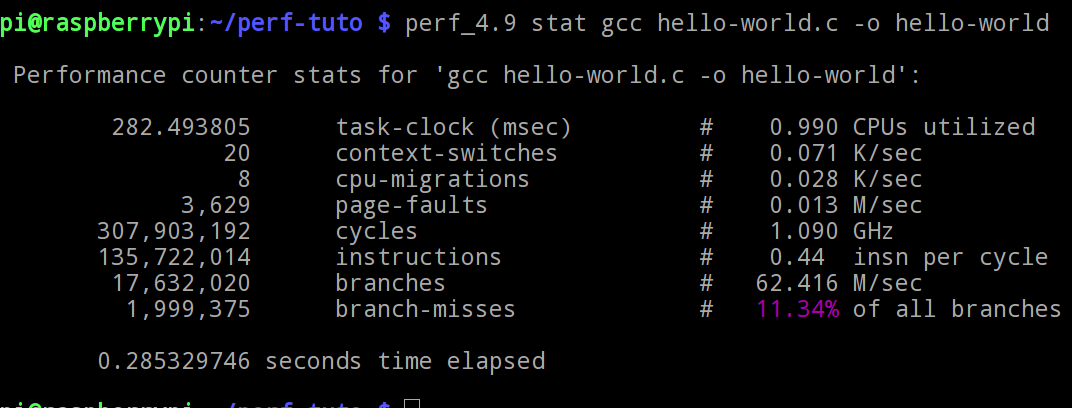
\includegraphics[scale=0.25]{img/solution/basic-statistics-using-perf.png}
        				\caption{Gather program's statistics - perf}
        				\label{Gather program's statistics - perf}
    				\end{figure}		
			
			
			\item \textbf{Filtering returned statistics : } one may choose which statistics to view as shown in \textbf{Figure \ref{Get specific program's statistics - perf}}.
					\begin{figure}[H]
						\centering
        				\includegraphics[scale=0.25]{img/solution/filter-statistics-using-perf.png}
        				\caption{Get specific program's statistics - perf}
        				\label{Get specific program's statistics - perf}
    				\end{figure}


		\end{enumerate}

	\item[$\bullet$] \textbf{Perf as a profiling tool : } perf can sample and record  applications callgraphs (or entire system).
	
	\begin{itemize}
		\item \textbf{record phase : } general syntax is shown below :
	\begin{lstlisting}[style=BashInputStyle]
# perf record -F <frequency_rate> [optional perf arguments] ./program [arguments_program]
	\end{lstlisting}	
	
	
An example is shown in \textbf{Figure \ref{Sampling function calls and stack traces on  the entire system}}.	
					\begin{figure}[H]
						\centering
        				\includegraphics[scale=0.4]{img/solution/record-hole-system-perf.png}
        				\caption{Sampling function calls and stack traces on  the entire system}
        				\label{Sampling function calls and stack traces on  the entire system}
    				\end{figure}
    				
    				
    	\item \textbf{Reading report : } reports can be read using :
 	\begin{lstlisting}[style=BashInputStyle]   	
    	$ sudo perf report -g	
    \end{lstlisting}	
Reports are displayed with functions sorted according to their execution time
(\textit{time exhaustive functions are on the top and shown in red})  as shown in \textbf{Figure \ref{Displaying Perf records in Basic mode}}.			
					\begin{figure}[H]
						\centering
        				\includegraphics[scale=0.4]{img/solution/basic-display-record-mode-perf.png}
        				\caption{Displaying Perf records in Basic mode}
        				\label{Displaying Perf records in Basic mode}
    				\end{figure}
 \textbf{Remark : } We can display a tree view report using : 
 	\begin{lstlisting}[style=BashInputStyle]   	
    	$ sudo perf report -g --stdio 
    \end{lstlisting} 
   				
    				
	\end{itemize}

	
	
	


	
	
	
	\item[$\bullet$] \textbf{Perf as a tracing tool : }
		\begin{enumerate}
			\item \textbf{Choose a tracepoint : } tracepoints must be supported by perf as shown in \textbf{Figure \ref{Check tracepoint support - perf}}.
					\begin{figure}[H]
						\centering
        				\includegraphics[scale=0.4]{img/solution/check-sched-switch-support-perf.png}
        				\caption{Check tracepoint sched\_switch support - perf}
        				\label{Check tracepoint support - perf}
    				\end{figure}		
			
			\item \textbf{Trace selected tracepoint events : } Launch our executable using perf (-e is used to select a tracepoint) as shown in \textbf{Figure \ref{trace sched-switch event - perf}}.
					\begin{figure}[H]
						\centering
        				\includegraphics[scale=0.4]{img/solution/trace-sched-switch-perf.png}
        				\caption{trace sched\_switch event - perf}
        				\label{trace sched-switch event - perf}
    				\end{figure}			
			
			\item \textbf{Read tracepoint report : } We can read the report using :
 	\begin{lstlisting}[style=BashInputStyle]   	
    	$ sudo perf script [-i Path_to_perf.data]
    \end{lstlisting} 			
An example is shown in \textbf{Figure \ref{Reading recorded sched-switch event - perf}}.
					\begin{figure}[H]
						\centering
        				\includegraphics[scale=0.25]{img/solution/read-perf-trace-sched-switch.png}
        				\caption{Reading recorded sched\_switch event - perf}
        				\label{Reading recorded sched-switch event - perf}
    				\end{figure}				
			
		\end{enumerate}
	

	\item {Hotspot : } A \textbf{GUI tool} for \textbf{Perf}, able to parse \og perf traces \fg or even make a recording.	An example is shown in \textbf{Figure \ref{Hotspot (a perf GUI tool) in action - generation of flame graphs}}.
		
					\begin{figure}[H]
						\centering
        				\includegraphics[scale=0.25]{img/solution/perf-hotspot.png}
        				\caption{Hotspot (a perf GUI tool) in action - generation of flame graphs}
        				\label{Hotspot (a perf GUI tool) in action - generation of flame graphs}
    				\end{figure}			
		
\textbf{Flame graphs : } Shows callgraph of stack frames. for instace, \og \_clone \fg frame calls \og start\_thread \fg frame in \textbf{Figure \ref{Hotspot (a perf GUI tool) in action - generation of flame graphs}}		
		
\end{itemize}


\subsubsection{eBPF}
BPF (\textit{Berkeley Packet Filter}) is the famous virtual machine (\textit{running inside the kernel}) which is used by {\color{blue}\url{https://www.tcpdump.org/}}.
eBPF (\textbf{Extended Berkeley Packet Filter}) is the extension of \textbf{BPF}. Hopefully, it does much more than handling packets, it can serve as an observality , DDos mitigation , Intrusion detection , Tracing , ..., etc ( \textbf{Figure \ref{Linux EBPF internal and usage}} - taken from Brenden Gregg's blog)
					\begin{figure}[H]
						\centering
        				\includegraphics[scale=0.4]{img/solution/security-monitoring-with-ebpf-11-638.jpg}
        				\caption{Linux EBPF internal and usage}
        				\label{Linux EBPF internal and usage}
    				\end{figure}	

eBPF is difficult to use (We must write C codes), BCC ( BPF Compiler Collection ) was made to make it easier.
BCC is a front-end toolkit of eBPF which can be found at the following page : {\color{blue}\url{https://github.com/iovisor/bcc}}.


\begin{enumerate}
	\item \textbf{Install bcc : } BCC became easy to install, instructions are provided at : {\color{blue}\url{https://github.com/iovisor/bcc/blob/master/INSTALL.md}}
	
	\item \textbf{Running eBPF scripts : } 
		\begin{itemize}
			\item \textbf{bcc provided scripts : } bcc ships with tools that handles everyday's common tasks. One can try them as shown in : {\color{blue}https://github.com/iovisor/bcc}
			
			\item \textbf{Creating scripts from scratch : } We can write custom eBPF scripts {\color{blue}\url{https://github.com/iovisor/bcc/blob/master/docs/tutorial_bcc_python_developer.md}}
						
			
		\end{itemize}			
\end{enumerate}

Basic syntax of eBPF : 

\begin{itemize}
	\item[$\bullet$] \textbf{Creating kprobe : } sample code is shown in \textbf{\color{red}Appendix {\color{blue}\ref{Attaching eBPF kprobe}}} (\textit{output result is illustrated in \textbf{Figure \ref{Tapping sys-mkdir using eBPF}}}).	
					\begin{figure}[H]
						\centering
        				\includegraphics[scale=0.4]{img/solution/sys_mkdir_detected.png}
        				\caption{Tapping sys\_mkdir using eBPF - kprobe}
        				\label{Tapping sys-mkdir using eBPF}
    				\end{figure}	
	
	
	\item[$\bullet$] \textbf{Creating tracepoint : } an example is shown in \textbf{\color{red}Appendix {\color{blue}\ref{Enabling eBPF Tracepoint}}} 	 (\textit{see \textbf{Figure \ref{Tapping module loading event using eBPF - tracepoint}}}).	
	
					\begin{figure}[H]
						\centering
        				\includegraphics[scale=0.4]{img/solution/creating-ebpf-tracepoint.png}
        				\caption{Tapping module loading event using eBPF - tracepoint}
        				\label{Tapping module loading event using eBPF - tracepoint}
    				\end{figure}		
	
	
\end{itemize}

\begin{center}
\fbox{
  \parbox{\textwidth}{
  	\begin{center}
	{\Large \textbf{\color{red}eBPF enhanced security}}\\
	 \textbf{eBPF} programs imposes restrictions (\textit{no infinite loops, kprobes cannot be attached to all functions, ..., etc}). It ensures that a script will never crash or hang kernel code ({\color{blue} \url{https://lkml.org/lkml/2015/4/14/232}}). 
	\end{center} 
  }
}
\end{center}


\textbf{\color{orange}Important : } Tracepoints are highly encouraged to be used than kprobes as they are more stable and portable (\textit{function names and prototype can change so kprobes will be incorrect}).
\subsubsection{Choosing a tracer}
The following table gives a quick summary of important features of some tracers :
\begin{center}
	\begin{tabular}{|c|c|c|c|c|c|}
		\hline
			\rowcolor{LightCyan}
			\textbf{Tool} & \textbf{Native} & \textbf{Front-end} & \textbf{Remote} & \textbf{GUI parsing} & \textbf{Real time} \\	
						\rowcolor{LightCyan}   
			 & \textbf{support} & \textbf{tool} & \textbf{tracing} & \textbf{tools} & \textbf{tracing} \\	 		
   		\hline
	    	\textbf{Ftrace} & since linux 2.7 & Trace-cmd & yes & KernelShark & no \\
	    \hline
	    	\textbf{Perf\_event} & since linux 2.8 & perf & no & Hotspot & no \\
		\hline     
        	\textbf{LTTng} & no & lttng & yes & Trace compass & no \\
		\hline     
        	\textbf{eBPF} & since linux 4.4 & bcc & no & no & no \\
   		\hline
	\end{tabular}
\end{center}

Tracers may be selected depending on requirements, We made a simple benchmarking tool to help us in choosing the most appropriate. The benchmark measures \textbf{memory} (\textit{captures Maximum Resident Set Size Memory}) and \textbf{execution time overhead} as well as other metrics (context switches and trace file size).

\begin{center}
\fbox{
  \parbox{\textwidth}{
  	\begin{center}
	{\Large \textbf{\color{red}Benchmarking sources}}\\
	 Sources are located at : {\color{blue}\url{https://github.com/jugurthab/Linux_kernel_debug/tree/master/DebugSoftware/tracers-cmp-benchmark}}.
	 
	 A python3 utility (available at : \textbf{\color{blue}\url{https://github.com/jugurthab/Linux_kernel_debug/tree/master/DebugSoftware/cmpTracer-GUI}}) visualizes the results in GUI form.
	\end{center} 
  }
}
\end{center}


Some results are shown below :
Tests were made 10 times (then average was taken) on a machine with initial conditions are shown in \textbf{Figure \ref{Target's initial state before experiment - Linux Mint}}

     		\begin{figure}[H]
					\centering
        			\includegraphics[scale=0.45]{img/solution/cmptracers-target-information.png}
        			\caption{Target's initial state before experiment - Linux Mint}
        			\label{Target's initial state before experiment - Linux Mint}
   			 \end{figure}
   			 
Results are shown as follow :
						\begin{center}
							\begin{tabular}{|c|c|c|c|c|c|c|}
								\hline
								\textbf{Tool} & \textbf{Execution} & \textbf{Max}  & \textbf{V.C} & \textbf{Inv.C} & \textbf{Minor page} & \textbf{Size of}\\
							& 	\textbf{time (s)} & \textbf{RSS} & \textbf{Switches} & \textbf{Switches} & \textbf{faults} & \textbf{file (KB)} \\
								   	
								\hline
	    						\textbf{qsort} & 0.19 & 8818 & 1 & 79 & 1194 &  0 \\								   		
   								\hline
	    						\textbf{Ftrace} & 4.04 & 8848 & 170 & 261 & 1323 & 29418  \\
								\hline     
        						
   								\textbf{Perf} & 0.53 & 10227 & 27 & 118 & 3170 & 23 \\
   								\hline
   								
   								\textbf{LTTng} & 0.21 & 8834 & 1 & 69 & 1213 & 2723 \\
   								\hline		
							\end{tabular}
						\end{center}


\textbf{\color{red}Important : } eBPF requires Linux4.9 to access full functionnalities (or at least Linux4.4 for partial support).

\subsection{Defeating Anti debugging mechanisms}
Security is a concern for every modern device, It became crucial to keep the data safe and avoid them from leaking.\\
Debugging is not only meant to troubleshoot a slow or faulty system. A good security analyst requires skills in debugging.\\
Bugs are not only introduced as a result of programming mistakes (No one writes perfect code), they can be caused by malicious code injected on purpose by attackers.

\subsubsection{Attacking userland}
Attacking the userland is a wide spread practice and requires only few setup to achieve the desired result.\\

The simplest example is the use of ptrace as shown below :
	\begin{lstlisting}[style=CStyle]
if(ptrace(PTRACE_TRACEME , 0) < 0 ){
     printf("You cannot debug me!\n");
     exit(EXIT_FAILURE);
}
    	\end{lstlisting}
The code snippet means that the process will be traced by it's father. \\

\textbf{\color{red}Problem : } only one debugger can be attached to a running process at time t (see \textbf{Figure \ref{GDB cannot attach to the program due to Anti-debugging}}).
    		\begin{figure}[H]
					\centering
        			\includegraphics[scale=0.45]{img/solution/gdb-cannot-be-attached.png}
        			\caption{GDB cannot attach to the program due to Anti-debugging}
        			\label{GDB cannot attach to the program due to Anti-debugging}
   			 \end{figure}
   			 As one can see from \textbf{Figure \ref{GDB cannot attach to the program due to Anti-debugging}}, GDB was not able to attach to the process (even if launched with root privileges).
   			 
\begin{center}
\fbox{
  \parbox{\textwidth}{
  	\begin{center}
	{\Large \textbf{\color{red}More attacks are possible}}\\
	Other methods have been experimented like : LD\_PRELOAD and hijacking C library ({\color{blue}\url{https://github.com/jugurthab/Linux_kernel_debug/tree/master/debug-examples/Chap6-kernel-security/userspace/LD_preload}}) 
	\end{center}	
  
  }
}
\end{center}
\subsubsection{Targeting Kernel Code}
The kernel can be subjected to many threats (like rootkits).
We can change behaviour of almost any instruction in the kernel (\textit{it's paramters and return value}), and cause
serious system issues that goes from simple \textbf{Denial of Services to steeling private data}.

Some basic attacks like : \textbf{Jprobes} ({\color{blue}\url{https://github.com/jugurthab/Linux_kernel_debug/tree/master/debug-examples/Chap6-kernel-security/kernel/jprobes}}) and \textbf{Kprobes} ({\color{blue}\url{https://github.com/jugurthab/Linux\_kernel\_debug/tree/master/debug-examples/Chap6-kernel-security/kernel/kprobes}}).


More advanced attacks like module tampering : ({\color{blue}\url{https://github.com/jugurthab/Linux_kernel_debug/tree/master/debug-examples/Chap6-kernel-security/kernel/module-tampering}})


\begin{enumerate}
	\item \textbf{Merge modules : } ld can assemble modules to produce a final one as shown in \textbf{Figure \ref{Meging modules using ld}}.
    		\begin{figure}[H]
					\centering
        			\includegraphics[scale=0.45]{img/solution/combining-modules-linux.png}
        			\caption{Meging modules using ld}
        			\label{Meging modules using ld}
   			 \end{figure}	
	
	
	
	\item \textbf{Analyse the resulting module :} We can dump module's symbol table of as follow :
\begin{lstlisting}[style=BashInputStyle]
$ objdump -t kernel-module-infected.ko
\end{lstlisting}

The reader can notice that \og fak\_module\_init \fg has been linked correctly.\\
All what is left is forcing \og init\_module \fg to point to our malicious symbol \og fak\_module\_init \fg (\emph{at relative location 00000014}).

\item \textbf{Make init\_module as an alias of fak\_module\_evil : } We must change the relative address of init\_module to execute our malicious function as shown below.
\begin{lstlisting}[style=BashInputStyle]
./elfchger -s init_module -v 00000014 kernel-module-infected.ko
\end{lstlisting}

Dumping the infected module using \og objdump -t kernel-module-infected.ko \fg is shown in \textbf{Figure \ref{Forcing init-module to become an alias of a malicious function}}

\begin{figure}[H]
					\centering
        			\includegraphics[scale=0.35]{img/solution/infected-module-dumped.png}
        			\caption{Forcing init\_module to become an alias of a malicious function}
        			\label{Forcing init-module to become an alias of a malicious function}
   			 \end{figure}
   			 

\item \textbf{Insert infected module into kernel : } see \textbf{Figure \ref{Infected module executing malicious function}}

\begin{figure}[H]
					\centering
        			\includegraphics[scale=0.35]{img/solution/hacked-module.png}
        			\caption{Infected module executing malicious function}
        			\label{Infected module executing malicious function}
   			 \end{figure}
   			 \begin{center}
   			 \color{red}
   			 The module is executing the evil function
   			 \end{center}
	
\end{enumerate}

\section{Encountered difficulties}
Debugging is a rare skill, only few resources are available. We can point out some difficulties that We have seen during internship :

\subsection{Hardware issues}
Hardware problems were a real bottlenecks, as they are more difficult to locate and troubleshoot.
\subsubsection{JTAG tampering}
Some manufacturers try to hide \textbf{JTAG connectors} to make it difficult to access (\textit{due to security reasons}). Beaglebone black wireless is an example of those boards. Soldering a JTAG connector was mandatory (\textit{it is not easy on those tiny devices}).

\textbf{\color{orange}Note : } sometimes JTAG connection is encrypted or even damaged by manufacturers (\textit{but this is rare}). 
More can be said about \textbf{JTAG} as connectors are different and pinout definition is not always easy to find (solutions like \textbf{JTAGulator} at : {\color{blue}\url{https://hackaday.com/2013/10/02/jtagulator-finds-debug-interfaces/}} may be helpful).
\subsubsection{OpenOCD hardware interfacing}
As mentionned previously, \textbf{OpenOCD} is a hardware debugging solution (it is complicated). It took me 1.5 week to understand how to make a correct hardware setup. Interfacing \textbf{OpenOCD} compliant adapter with the target is far to be easy (\textbf{Figure \ref{OpenOCD ACK error due to incorrect TDI connection}}).


\begin{figure}[H]
		\centering
        \includegraphics[scale=0.40]{img/issues/tdi-not-connected-openocd.png}
        \caption{OpenOCD ACK error due to incorrect TDI connection}
        \label{OpenOCD ACK error due to incorrect TDI connection}
    \end{figure}


\subsubsection{OpenOCD's compliant adapter}
Adapters are expensive, adapters that are compatible with OpenOCD are difficult to find.\\
\textbf{Solution : } We used ARM-USB-TINY-H ({\color{blue} \url{https://www.olimex.com/Products/ARM/JTAG/ARM-USB-TINY-H/}}) from Olimex.

\subsection{Software}

\subsubsection{Debugging symbols}
Most kernels in production are compiled stripping this option. The advantage is to reduce kernel's image size, however, tools like : GDB becomes practically useless as they require debugging symbols (see \textbf{Figure \ref{GDB is practically useless without debugging symbols}}). 

\begin{figure}[H]
		\centering
        \includegraphics[scale=0.40]{img/issues/no-debug-symbol.png}
        \caption{GDB is practically useless without debugging symbols}
        \label{GDB is practically useless without debugging symbols}
    \end{figure}


Some solutions exist to reconstruct it (without recompiling the kernel) but works only fine on x86 (see {\color{blue}\url{https://github.com/elfmaster/kdress}}).




Even worse, /proc/kcore does not exist on most embedded systems (like ARM)\footnote{More details about /proc/kcore are available at :  {\color{blue}\url{https://lwn.net/Articles/45315/}}}.


\subsubsection{Yama blocks ptrace}
Yama is a security module that disables ptrace. GDB, strace and ltrace make use of ptrace which must be enabled.\\

\textbf{\color{orange}Solution : } enable ptrace as shown in {\color{red}subsection {\color{blue}\ref{System calls and library calls}}}
\subsubsection{JTAG lockers}
Even if OpenOCD's hardware interfacing is correct, some boards have software protections to disable JTAG. Raspberry PI is an example. The firmware blocks any JTAG connection by default. Workarounds were made to disable such mechanisms.\\

\textbf{\color{orange}Solution : } enable JTAG as shown in {\color{red}subsection {\color{blue}\ref{Linux hardware debugging with OpenOCD}}}
\subsubsection{Disabled serial communication}
Serial communication can be disabled on some devices, \textbf{Raspberry PI} is an example of those. It took me 3 hours to figure out the reason of unsuccessful connection (\textit{even if hardware setup is correct} as shown in \textbf{Figure \ref{Hardware setup for serial communication - Raspberry PI 3}}). 


\begin{figure}[H]
		\centering
        \includegraphics[scale=0.40]{img/issues/USB-Serial-cable-To-Raspberry-PI-3_bb.png}
        \caption{Hardware setup for serial communication - Raspberry PI 3}
        \label{Hardware setup for serial communication - Raspberry PI 3}
    \end{figure}



\textbf{\color{orange}Solution : } To enable serial communication on Raspberry PI, follow the steps presented at : {\color{blue}\url{https://hallard.me/enable-serial-port-on-raspberry-pi/}}.
\subsubsection{OpenOCD scripts}
As We have already mentionned, OpenOCD does not support every board. Custom configuration files must be written to include new platforms. We have made scripts generation easier with OESdebug, provided step by step documentation of OpenOCD and an animation that helps to understand more ({\color{blue} \url{https://jugurthab.github.io/debug_linux_kernel/zero-to-hero-openocd.html}}).\\

{\color{orange}Solution : } see {\color{red}subsection {\color{blue}\ref{Linux hardware debugging with OpenOCD}}} (go to \og \textit{OpenOCD made easy with OESdebug} \fg).


\subsubsection{DebugFs absent}
Security engineers drop down \textbf{DebugFs} support as it allows anyone to get insight into the Kernel. Only Hardware debugging can help in such case.\\
We point the fact that tracers will be difficult to port and used as some rely heavily on \textbf{DebugFS}.


\section{Conclusion}
 A long journey was made with Linux debugging, testing tools and documenting results. We have crossed through the userspace, then went exploring various tools like : \emph{GDB}, \emph{Valgrind}, \emph{strace} and \emph{ltrace}.\\

We moved to Kernel-land and learnt to solve it's issues through debuggers (KGDB/KDB, Kernel oops and Magic SysRq). We provided a step by step guide for writing custom OpenOCD scripts for JTAG debugging (We also have made a wrapper tool to make it easier). 

We also made a big step in understanding Linux working internals with tracers (Ftrace, Perf, LTTng). We have seen their usages, front-end tools and compared them to help us choosing the most appropriate for a given situation. We have also discovered eBPF which is the most prominent Linux tracer.
\vspace{10px}
We must keep in mind that debugging is not only made to trace bugs, but also reverse malicious code (another reason to sharpen our debugging skills). Such scenarios are quite common today, and being able to detect them is a crucial requirement.

\vspace{5px}
Once again, We should stress out that debugging can save hours of trying to troubleshoot a problem. We must keep in mind that developpers work in team, each has it's coding style and not everyone checks for return values, null pointers, buffer overflows, ..., etc.



\vspace{7px}
Reader must keep in mind that printf(printk) works great with small codes, however can overwhelm a system with messages, making it slow and even unresponsive. Industrial projects can goes beyond of million lines of code.\\



\begin{center}
\color{red}
Personally, I enjoyed SMILE's internship, It prepared me for real world industry and tought me that we need more than coding skills to be a good developper.  I had a lot of fun debugging Linux, gathering performances and stack traces and I loved OpenOCD as Hardware JTAG debugging allows a complet control over target.
\end{center}






\begin{appendices}

\section{eBPF}
\subsection{Attaching eBPF kprobe}
\label{Attaching eBPF kprobe}

\begin{lstlisting}[style=PythonStyle]
from bcc import BPF

# prog will store the eBPF C program
prog = """
int detect(void *ctx){
	// write message into trace_pip
	bpf_trace_printk("sys_mkdir detected!\\n");
	return 0; // always return 0
}
"""

# Loads eBPF program
b = BPF(text=prog)

# Attach kprobe to kernel function and sets  ... as jprobe handler
b.attach_kprobe(event="sys_mkdir", fn_name="detect")

# Show message when ePBF stats
print("Detection stated .... Ctrl-C to end")

# print result to user
while 1:
	# read messages from trace_pip and display them to user
	b.trace_print()
\end{lstlisting}



\subsection{Enabling eBPF Tracepoint}
\label{Enabling eBPF Tracepoint}
\begin{lstlisting}[style=PythonStyle]
from bcc import BPF

# prog will store the eBPF C program
prog = """
TRACEPOINT_PROBE(module, module_load){
	// events are from /sys/kernel/debug/tracing/events/module/module_load/format 
	bpf_trace_printk("Module has been loaded!\\n");
	return 0; // always return 0
};
"""

# Loads eBPF program
b = BPF(text=prog)

# Show message when ePBF stats
print("Loading module snooping stated .... Ctrl-C to end")

# print result to user
while 1:
	# read messages from trace_pip and display them to user
	b.trace_print()
\end{lstlisting}



\end{appendices}


\end{document}